% Customizable fields and text areas start with % >> below.
% Lines starting with the comment character (%) are normally removed before release outside the collaboration, but not those comments ending lines

% svn info. These are modified by svn at checkout time.
% The last version of these macros found before the maketitle will be the one on the front page,
% so only the main file is tracked.
% Do not edit by hand!
\RCS$Revision: 494080 $
\RCS$HeadURL: svn+ssh://svn.cern.ch/reps/tdr2/papers/HIG-18-021/trunk/HIG-18-021.tex $
\RCS$Id: HIG-18-021.tex 494080 2019-04-24 06:20:00Z rverma $
%%%%%%%%%%%%% local definitions %%%%%%%%%%%%%%%%%%%%%
% This allows for switching between one column and two column (cms@external) layouts
% The widths should  be modified for your particular figures. You'll need additional copies if you have more than one standard figure size.
\newlength\cmsFigWidth
\ifthenelse{\boolean{cms@external}}{\setlength\cmsFigWidth{0.49\textwidth}}{\setlength\cmsFigWidth{0.65\textwidth}} % example: one column in journal, 2/3 in CMS
\ifthenelse{\boolean{cms@external}}{\providecommand{\cmsLeft}{upper\xspace}}{\providecommand{\cmsLeft}{left\xspace}}
\ifthenelse{\boolean{cms@external}}{\providecommand{\cmsRight}{lower\xspace}}{\providecommand{\cmsRight}{right\xspace}}


%%%%%%%%%%%%%%%  Title page %%%%%%%%%%%%%%%%%%%%%%%%
\cmsNoteHeader{HIG-18-021} % This is over-written in the CMS environment: useful as preprint no. for export versions

\newcommand{\Hp}{\ensuremath{\PH^+}\xspace}
\newcommand{\Hn}{\ensuremath{\PH^-}\xspace}
\newcommand{\ttjets}{\ensuremath{\ttbar + \text{jets}}\xspace}
\newcommand{\mjj}{\ensuremath{m_\text{jj}}\xspace}
\newcommand{\mt}{\ensuremath{m_{\PQt}}\xspace}
\providecommand{\cmsTable}[1]{\resizebox{\textwidth}{!}{#1}}
\renewcommand{\arraystretch}{1.2}
\title{Search for a light charged Higgs boson in the H$^{\pm} \rightarrow$ cs channel at 13 TeV}

\address[tifr]{Tata Institute of Fundamental Research, Mumbai, India}
\address[IOP]{Institute of Physics, Bhubaneswar, India}
\address[UCSD]{University of California San Diego, USA}
\author[tifr]{S.R.~Dugad}
\author[UCSD]{G.~Kole}
\author[tifr]{G.B.~Mohanty}
\author[IOP]{A.~Nayak}
\author[tifr]{R.K.~Verma}

\date{\today}

\abstract{
A search is conducted for a low-mass charged Higgs boson produced in a top quark decay and subsequently decaying into a charm and an antistrange quark. The data sample was recorded in proton-proton collisions at $\sqrt{s}=13~\mathrm{TeV}$ by the CMS experiment at the LHC and corresponds to an integrated luminosity of $35.9~\mathrm{fb}^{-1}$. The signal search is conducted in the process of top-quark pair production, where one top quark decays to a bottom quark and a charged Higgs boson, and the other to a bottom quark and a W boson. With the W boson decaying to a charged lepton (electron or muon) and a neutrino, the final state comprises an isolated lepton, missing transverse momentum, and at least four jets, of which two are tagged as b jets. To enhance the search sensitivity, one of the jets originating from the charged Higgs boson is required to satisfy a charm tagging requirement. No significant excess beyond standard model predictions is found in the dijet invariant mass distribution. An upper limit in the range $0.20$$-$$1.65\%$ is set on the branching fraction of the top quark decay to the charged Higgs boson and bottom quark for a Higgs mass between $80$ and $160$ GeV.
}
\hypersetup{%
pdfauthor={S.R. Dugad, G. Kole, G.B. Mohanty, A. Nayak, R.K. Verma},%
pdftitle={Search for a light charged Higgs boson in the H$^{\pm} \rightarrow$ cs channel at 13 TeV},%
pdfsubject={CMS},%
pdfkeywords={CMS, physics, charged Higgs boson, MSSM}}
\maketitle

\newpage
%%%%%%%%%%%%%%%%%%%%%%% INTRODUCTION %%%%%%%%%%%%%%%%%%%%%%%
\label{s:secIntro}
The discovery of the Higgs boson in 2012 by the CMS~\cite{Chatrchyan:2012ufa}
and ATLAS~\cite{Aad:2012tfa} experiments at the CERN LHC has ushered in a new
beginning in the field of particle physics. The Higgs boson could be the first
of many elementary scalars present in nature to be observed
in the laboratory. Various extensions to the standard model (SM), such as
supersymmetry~\cite{Martin:1997ns,Golfand:1971iw,Wess:1974tw} and the two
Higgs doublet model (2HDM)~\cite{Branco:2011iw}, predict multiple scalars
as the remnants of an additional SU(2)$_L$ complex doublet introduced to
address some known limitations of the SM. After spontaneous symmetry breaking,
out of the eight degrees of freedom of the two Higgs doublets, three are used
to make the \PW and \PZ bosons massive, leaving five physical scalar
particles. Of these, two (\Ph, \PH) are neutral Higgs bosons which are
CP-even (scalar), one (\PSA) is neutral and CP-odd (pseudoscalar), and the
remaining two are charged Higgs bosons \PHpm.

The 2HDM can be classified into different categories depending on the type of
interaction of the two doublets with quarks and charged leptons. For example,
in the type I 2HDM, fermions have Yukawa couplings only to the second doublet.
The nature of the Yukawa coupling determines the branching fraction of the charged
Higgs boson decays into different final states. We are interested in the decay
channel $\PSHp \to \PQc\PAQs$ (and its charge conjugate), whose branching fraction
can range up to 100\%, depending on the type of Yukawa couplings. The
latter is expressed in terms of the parameter $\tan\beta=v_2/v_1$, where $v_1$ and
$v_2$ are the vacuum expectation values of the two Higgs doublets. In the minimal
supersymmetric standard model (MSSM), this is the dominant decay channel for low values of
$\tan\beta$~\cite{Aoki:2009ha}.
In this analysis, we assume that $\mathcal{B}(\PSHp \to \PQc\PAQs) = 100$\%.

There have been many earlier searches for charged Higgs bosons at LEP, the Tevatron, and
the LHC. At LEP, it was expected to be dominantly produced by the process $\Pep\Pem \to \PSHp\PSHm$.
The search was conducted by assuming that \PSHp decays only to $\PQc\PAQs$ and
$\Pgt\Pagngt$. Assuming that the sum of the branching fractions
$\mathcal{B}(\PSHp \to \Pgt^+\Pgngt) +\mathcal{B}(\PSHp \to \PQc\PAQs)=1$,
a lower limit of 79.3\GeV was obtained for the charged Higgs mass at
95\% confidence level (CL)~\cite{Achard:2003gt, Heister:2002ev, Abdallah:2003wd}.
Under a more general assumption $\mathcal{B}(\PSHp \to \Pgt^+\Pgngt) +
\mathcal{B}(\PSHp \to \PQq\PAQq^\prime)=1$, a slightly less stringent
constraint of 76.3\GeV was obtained at 95\% confidence level~\cite{Abbiendi:2008aa}.

Limits on charged Higgs production at hadron colliders have been set by the Tevatron and LHC,
assuming the production mode $\PQt \to \PSHp\PQb$. The CDF
collaboration~\cite{Aaltonen:2009ke} set a 95\% \CL upper limit on the
branching fraction $\mathcal{B}(\PQt \to \PSHp\PQb)$ of 10--30\% for a charged
Higgs lying in the mass range 60--150\GeV, assuming that $\PSHp$ decays dominantly
to $\PQc\PAQs$. Similar limits have been obtained by the D0
experiment~\cite{Abazov:2009aa}. Using 7\TeV data, the ATLAS Collaboration set an upper
limit at 95\% \CL on the product $\mathcal{B}(\PQt \to \PSHp\PQb)
\mathcal{B}(\PSHp \to \PGtp\PGn)$ of 0.23--1.3\% for a charged Higgs mass
in the range 80--160\GeV~\cite{Aad:2013hla}. A search for a charged Higgs
boson decaying into $\PQc\PAQs$ was performed with 8\TeV data by the CMS Collaboration, which set
an upper limit at 95\% \CL on $\mathcal{B}(\PQt \to \PSHp\PQb)$ in the range
1.2--6.5\%~\cite{Khachatryan:2015uua}.

As illustrated in Fig.~\ref{fig:feyn_diag_sig}, in the signal process for \PSHp production, one of
the top quarks decays to $\PSHp\PQb$ and the other to $\PWm\PAQb$, with \PSHm production proceeding
by the charge conjugate of this process. The principal
SM background to this search consists of \ttbar pair production where one of the
top quarks decays by $\PQt \to \PWp\PQb$ and the other top quark decays by
$\PAQt \to \PWm\PAQb$. The $\PWp/\PSHp$ decays hadronically into ``light'' jets (not
from a \PQb quark), whereas the \PWm decays leptonically (in the \ttbar case, this
is called the ``semileptonic'' decay channel); we define two channels depending on whether
the lepton produced in the \PWm decay is an electron or a muon (events with tau
leptons are not considered).
\begin{figure}[htp]
\centering
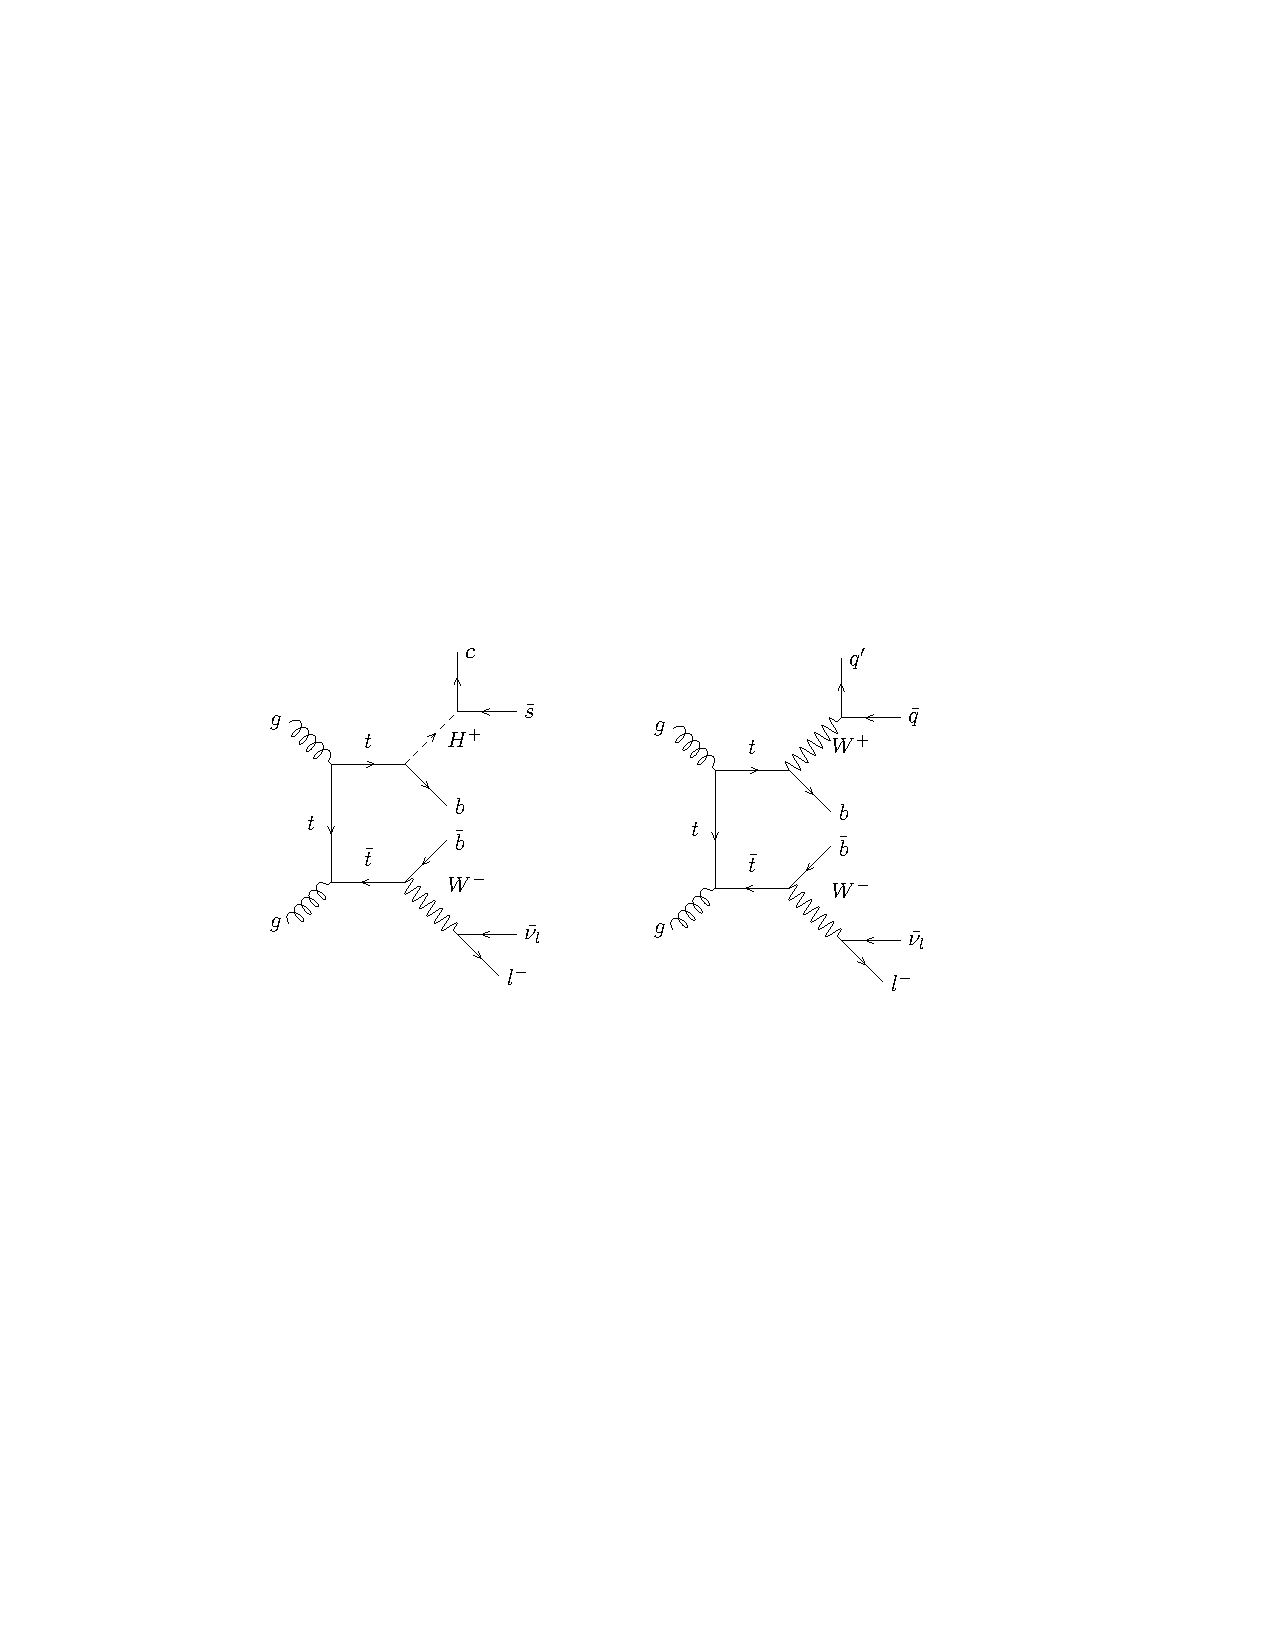
\includegraphics[width=0.75\textwidth]{Image/feyn_diag_sig.pdf}
\caption{Production of \ttbar from gluon-gluon scattering. The left plot
    shows the signal process in which the \ttbar pair decay products include
    a charged Higgs boson. The right plot shows the SM decay of the \ttbar pair
    in the semileptonic decay channel.}
\label{fig:feyn_diag_sig}
\end{figure}

%////////////////////////// THE CMS DETECTOR /////////////////////////////
\section{The CMS detector}
\label{s:secCMS}
The central feature of the CMS apparatus is a superconducting solenoid of 6\unit{m}
internal diameter, providing a magnetic field of 3.8\unit{T}. Within the solenoid volume
are a silicon pixel and strip tracker, a lead tungstate crystal electromagnetic
calorimeter (ECAL), and a brass and scintillator hadron calorimeter (HCAL), each
composed of a barrel and two endcap sections. Silicon pixel and tracker detector
identifies the trajectory of charged particles and accurately measures their transverse
momentum up to $|\eta| \leq 2.5$.  Forward calorimeters extend the pseudorapidity
coverage provided by the barrel and endcap calorimeter. Segmented calorimeters
provide sampling of electromagnetic and hadronic showers up to $|\eta| \leq 5$.
Muons are detected in gas-ionization chambers embedded in the steel flux-return
yoke outside the solenoid in the range of $|\eta| \leq 2.4$. Events of interest
are selected using a two-tiered trigger system~\cite{Khachatryan:2016bia}. The
first level (L1), composed of custom hardware processors, uses information from
the calorimeters and muon detectors to select events at a rate of around
100\unit{kHz} within a time interval of less than 4\mus. The second level, known
as the high-level trigger (HLT), consists of a farm of processors running a
version of the full event reconstruction software optimized for fast processing,
and reduces the event rate to around 1\unit{kHz} before data storage. A more
detailed description of the CMS detector, together with a definition of the coordinate
system used and the relevant kinematic variables can be found~\cite{Chatrchyan:2008zzk}.

%% ////////////////////////// MC and data samples ///////////////////
\section{Data and simulation}
\label{s:secDataMC}
The data used for the analysis was collected by the CMS detector in 2016 in proton-proton ($\Pp\Pp$)
collisions at $\sqrt{s} = 13\TeV$, with an integrated luminosity of 35.9\fbinv.
The events selected online require, at the L1 trigger level, a muon candidate with $\pt > 22\GeV$ or an
electron or photon candidate with $\pt > 30\GeV$, or 22\GeV if it is isolated; at the HLT level, an isolated
muon (electron) with $\pt > 24$ (27)\GeV is required.

As shown in Fig.~\ref{fig:feyn_diag_sig}, the charged
Higgs is assumed to decay into $\PQc\PAQs$ or $\PAQc\PQs$ only. As a result, in the final state,
there will be four jets (two \PQb jets, one \PQc jet, one \PQs jet), one lepton (\Pe or \Pgm;
\Pgt is not considered in this analysis) and missing transverse momentum (\ptmiss), which is
attributed to the neutrino.
The SM processes that give the same final states (four jets + one lepton + missing
transverse momentum) are considered as background channels for this analysis. The
simulated signal and background samples are generated
using the \MGvATNLO~\cite{Alwall:2014hca} and \POWHEG
v2~\cite{Frixione:2007vw, Nason:2004rx, Alioli:2010xd} generators at parton
level. In all cases, these parton level events are hadronized using \PYTHIA
8~\cite{Sjostrand:2007gs} with the
CUETP8M1~\cite{Khachatryan:2015pea} tune, and then passed
to \GEANTfour~\cite{Agostinelli:2002hh} for simulation of the CMS detector response. Finally, the events
are reconstructed after complete detector simulation using the same
reconstruction process as for data.

The SM \ttjets process is an irreducible background, and represents the largest contribution,
about 94\% of the total expected background in the signal region.
The parton level SM \ttjets events are generated using \POWHEG v2
at next-to-leading order (NLO)~\cite{Campbell:2014kua}. The NNPDF30\_nlo\_as\_0118~\cite{Ball:2017nwa}
PDF set is used for this purpose. The events are hadronized and simulated as
above. The next-to-NLO cross-section for $\ttjets$ is estimated to be
$831.76 \pm^{20}_{29}(\text{scale}) \pm 35\,(\text{PDF}
+ \alpS)$\unit{pb}~\cite{Beneke:2011mq}. For simplicity, the top quark mass is
taken to be 172.5\GeV.

The charged Higgs signal samples are generated using \MGvATNLO. Only \PSHp samples are generated, and
\PSHm production is assumed to be the same. The
signal sample is generated for several mass points in the range of 80 to 160\GeV (80, 90, 100,
120, 140, 150, 155, and 160\GeV). The cross section
for the signal is $831.76 \times 0.21$\unit{pb}, where 831.76\unit{pb} is the inclusive SM
$\ttjets$ production cross section and the factor of 0.21 is the branching
fraction of $\PWm \to \ell^- \PAGn_\ell$ (where $\ell$ =
\Pe or \Pgm)~\cite{Tanabashi:2018oca}. Furthermore, the signal events are scaled by
a factor of $2\times 0.065\times (1-0.065) = 0.12$, where 6.5\% is the maximum observed
upper limit on $\mathcal{B}(\PQt \to \PSHp\PQb)$ obtained at 8\TeV~\cite{Khachatryan:2015uua}.

The single top quark production processes, where a top quark is produced with
jets in the s-channel, t-channel, or tW-channel, can also mimic the signal
topology. The s-channel single top production samples are generated
using \MGvATNLO~\cite{Alwall:2014hca}, while the t-channel and tW-channel
samples are generated using \POWHEG~\cite{Alioli:2009je,Re:2010bp}. The production of \PW and \PZ bosons with
jets, and vector boson fusion, are also considered as background
processes. The inclusive $\PW + \text{jets}$
and $\PZ/\PGg + \text{jets}$ samples are generated using
\MGvATNLO, with the MLM technique~\cite{Alwall:2007fs} used to avoid double counting. The vector boson fusion samples
($\PW\PW/\PW\PZ/\PZ\PZ$, collectively referred to as ``VV'') are generated using \PYTHIA 8.

Furthermore, SM events containing only jets produced through the strong
interaction, referred to as quantum chromodynamics (QCD) multijet events, can
also produce a final state identical to the signal topology, even though these
events contain only quarks at the parton level. QCD multijet events can have
reconstructed leptons from the misidentification of bottom and
charm hadrons, and \ptmiss due to the poor measurement of hadronic activity
inside the CMS detector. The simulation of QCD multijet events is
computationally intensive, resulting in a limited number of such events being
available. Because of this lesser number of events compared to the cross
section, the statistical uncertainty is high. Also, the simulated QCD multijet
events are not well modeled for high jet multiplicities. In view of this, a
data-driven approach is used to make a more precise estimation of the QCD
multijet background.

With the exception of the QCD multijet background, the expected yield for each
background process is determined from simulation. For the QCD multijet background,
a method known as the ``ABCD method'' is used. First, a normalization is determined
from the (low \ptmiss, isolated) and (low \ptmiss, anti-isolated) regions; then,
the QCD shape is determined from the (high \ptmiss, anti-isolated) region. By
using the normalization obtained on the shape, the expected QCD multijet
contribution is determined in the signal region (high \ptmiss, isolated). The
low and high \ptmiss regions are defined by \ptmiss $<$ 20 GeV and \ptmiss $>$
20 GeV, respectively. In the muon channel, the isolated and anti-isolated regions
are defined by $I_\text{rel}^\mu < 0.15$ and $0.15 < I_\text{rel}^\mu < 0.4$, where
$I_\text{rel}$ is the relative isolation variable. The relative isolation of a lepton is
defined as the ratio of the sum of $\pt$ for all the other particles to the $\pt$ of
the corresponding lepton within a cone of $\Delta R = \sqrt {\Delta \eta^2 + \Delta \phi^2} = 0.4$ around the lepton.
For the electron channel, the isolated region corresponds to $I_\text{rel}^e <$ 0.08 (0.07) and the
non-isolated region to 0.08 $< I_\text{rel}^e <$ 0.3 (0.07 $< I_\text{rel}^e <$ 0.3) for electrons in the barrel (endcap) regions.

%% ////////////////////////// Physics Object reconstruction ///////////////////
\section{Event reconstruction}
\label{s:secReco}
The physics objects of interest are mainly leptons, jets, missing
transverse momentum, vertices of pp collisions, and displaced vertices from the decay of
bottom or charm hadrons. The particle flow (PF) algorithm~\cite{Sirunyan:2017ulk}
is used to reconstruct these objects by optimally using various subsystems of
the CMS detector.

%--------------------------------------
% Primary-vertex reconstruction
%--------------------------------------
The collision vertices are obtained using reconstructed tracks in the silicon
tracker. First, candidate vertices are obtained by clustering tracks using the
deterministic annealing algorithm~\cite{Rose:1998dzq}.  Subsequently,
candidate vertices with at least two tracks are fitted using the adaptive
vertex fitter~\cite{Fruhwirth:1027031}. A primary vertex associated with a hard interaction is expected to be
accompanied by a large number of tracks.

The reconstructed vertex with the largest value of summed physics-object $\pt^2$ is taken to be the primary
$\Pp\Pp$ interaction vertex. The physics objects are the jets, clustered using the jet finding
algorithm~\cite{Cacciari:2008gp,Cacciari:2011ma} with the tracks assigned to the vertex as inputs, and the
associated missing transverse momentum, taken as the negative vector sum of the \pt of those jets.
Further, the reconstructed primary vertex is required to be within 24\unit{cm} along the beam axis and
within 2\unit{cm} in the transverse direction from the nominal $\Pp\Pp$ interaction region.


%--------------------------------------
% Electron Reconstruction
%--------------------------------------
Electrons are reconstructed using the PF algorithm~\cite{Sirunyan:2017ulk}
based on the tracks in the tracker and energy deposits in the electromagnetic
calorimeter~\cite{Khachatryan:2015hwa}. The reconstructed trajectory in the
tracker is mapped to the energy deposit in the ECAL to form an electron candidate.
The bending direction of the trajectory in the tracker is used to identify the charge of an electron.

%--------------------------------------
% Muon Reconstruction
%--------------------------------------
Muons, being minimum ionising particles, can traverse a long distance in the CMS
detector. The trajectory of the muon is bent due to the presence of a strong
magnetic field inside the solenoid and the return magnetic field in the opposite
direction outside the solenoid. Muon candidates are identified in the muon detectors and matched to tracks measured in the silicon tracker, resulting in an excellent \pt resolution between 1 and 10\% for \pt values up to 1\TeV.

%--------------------------------------
% Jet Reconstruction
%--------------------------------------
Due to color confinement~\cite{Polyakov:1976fu}, the quarks and gluons produced
in pp collisions cannot exist in free states; instead, they produce a cluster
of colorless hadrons, which subsequently decay to leptons and photons. Jets are
clustered from the reconstructed particle-flow candidates using the anti-\kt
algorithm~\cite{Cacciari:2008gp,Cacciari:2011ma} with a distance parameter of
$\Delta R = 0.4$. Each jet is required to pass
dedicated quality criteria to suppress the impact of instrumental noise and
misreconstruction.
Additional proton-proton interactions within the same or nearby bunch crossings (pileup) can contribute
additional tracks and calorimetric energy depositions, increasing the apparent jet momentum. To mitigate this
effect, tracks identified to be originating from pileup vertices are discarded and an offset correction is
applied to correct for remaining contributions. Jet energy corrections are derived from simulation studies so
that the average measured response of jets becomes identical to that of particle level jets. In situ
measurements of the momentum balance in dijet, $\PGg+\text{jet}$, $\PZ+\text{jet}$, and multijet events are
used to determine any residual differences between the jet energy scale in data and in simulation, and
appropriate corrections are made~\cite{Khachatryan:2016kdb}.

%--------------------------------------
% ptmiss Reconstruction
%--------------------------------------
The missing transverse momentum vector \ptvecmiss is defined as the projection onto the
plane perpendicular to the beam axis of the negative vector sum of the momenta of all reconstructed
particle-flow objects in an event. Its magnitude is referred to as \ptmiss. Neutrinos, being weakly
interacting particles with a very low cross section, cannot be directly detected
by the CMS detector and thus contribute to \ptmiss. The \ptmiss in the simulation and data
can have different resolutions. Therefore, in simulated events the \ptmiss value is smeared by propagating
the jet energy corrections to \ptmiss.

%--------------------------------------
% b/c Tagging
%--------------------------------------
There are two \PQb jets in the final state illustrated in Fig.~\ref{fig:feyn_diag_sig}
in both the charged Higgs signal process and the SM $\ttbar$+jets background. An accurate
identification of \PQb jets substantially reduces the SM backgrounds from other processes
such as $\PZ/\PGg + \text{jets}$, VV, $\PW + \text{jets}$, etc. The combined
secondary vertex (CSVv2) method~\cite{Chatrchyan:2012jua} is used to tag a
\PQb jet. The algorithm combines information on track impact parameters and
secondary vertices within a jet into an artificial neural network classifier
that provides separation between a \PQb jet and jets of other flavors. As the
charged Higgs boson decays to a charm and an antistrange quark, the
identification of charm jets is expected to increase the signal significance.
A charm tagger has been recently developed~\cite{CMS-PAS-BTV-16-001}
for 13\TeV data. It is based on the CSVv2 method and works similarly to the \PQb tagging procedure.


%%%%%% EVENT SELECTION %%%%%%%%%%%
\section{Event selection}
\label{s:secEvtSel}
In the event topology of interest, there are four jets (two \PQb jets and two light
jets), one charged lepton, and \ptmiss. Various selection requirements are applied to
ensure the resulting events have this topology. In the
offline analysis, events that pass the previously described triggers and contain a muon (electron) with $\pt > 26$ (30)\GeV
and $|\eta| <$ 2.4 (2.5) are selected. The signal event topology has only one lepton, so events having a second lepton with $\pt^\ell > 15$\GeV are rejected.
To eliminate events where the lepton is found within a jet, a requirement on the relative isolation is used.
This requirement is $I_\text{rel}^{\mu} < 0.15$ for muons, and
$I_\text{rel}^e < 0.08 (0.07)$ for electrons in the barrel (endcap) region.
No charge requirement is applied to the lepton.

Jets are selected by requiring $\pt^\text{j} > 25$\GeV, $|\eta^\text{j}| < 2.4$, neutral hadron energy
fraction $<$ 0.99, neutral electromagnetic energy fraction $<$ 0.99, number of
constituents $>$ 1, charged hadron energy fraction $>$ 0, charged hadron multiplicity $>$ 0, and charged
hadron electromagnetic energy fraction $<$ 0.99, where more details about these can be found in
Ref.~\cite{Sirunyan:2017ulk}; a total of at least four jets is required.
The \ptmiss is required to be greater than 20\GeV. The events are required to have at least
two \PQb jets satisfying the medium \PQb tagger working point
(discriminant value $>$ 0.8484)~\cite{Chatrchyan:2012jua}. The corresponding \PQb tagging efficiency is
63\% and the probability of a light jet being misidentified as a \PQb jet is 1\%.


%--------------------------------------
% Kinematic Fitting
%--------------------------------------
\section{Dijet invariant mass (\texorpdfstring{\mjj}{mjj}) distribution}
In this analysis, the charged Higgs boson is assumed to decay to $\PQc\PAQs$ or $\PAQc\PQs$. The invariant mass of the system
of the two light jets (\mjj) is thus used as the final observable. The \mjj distribution of the two
highest \pt light jets is shown in the top row of Fig.~\ref{fig:mjjBTagKinFit} for the two channels. If the
two observed light jets come from a semileptonic \ttbar decay, then the \mjj distribution should have a peak
at the \PW boson mass. However, the observed mean of the \mjj distribution is much higher (around 138\GeV),
reflecting the fact that the two light jets in each event may not necessarily come from the decay of a \PW
boson. In addition, the \mjj distribution has a long tail, which might constrain the search for new resonances
in the dijet mode.

\begin{figure}
    \centering
    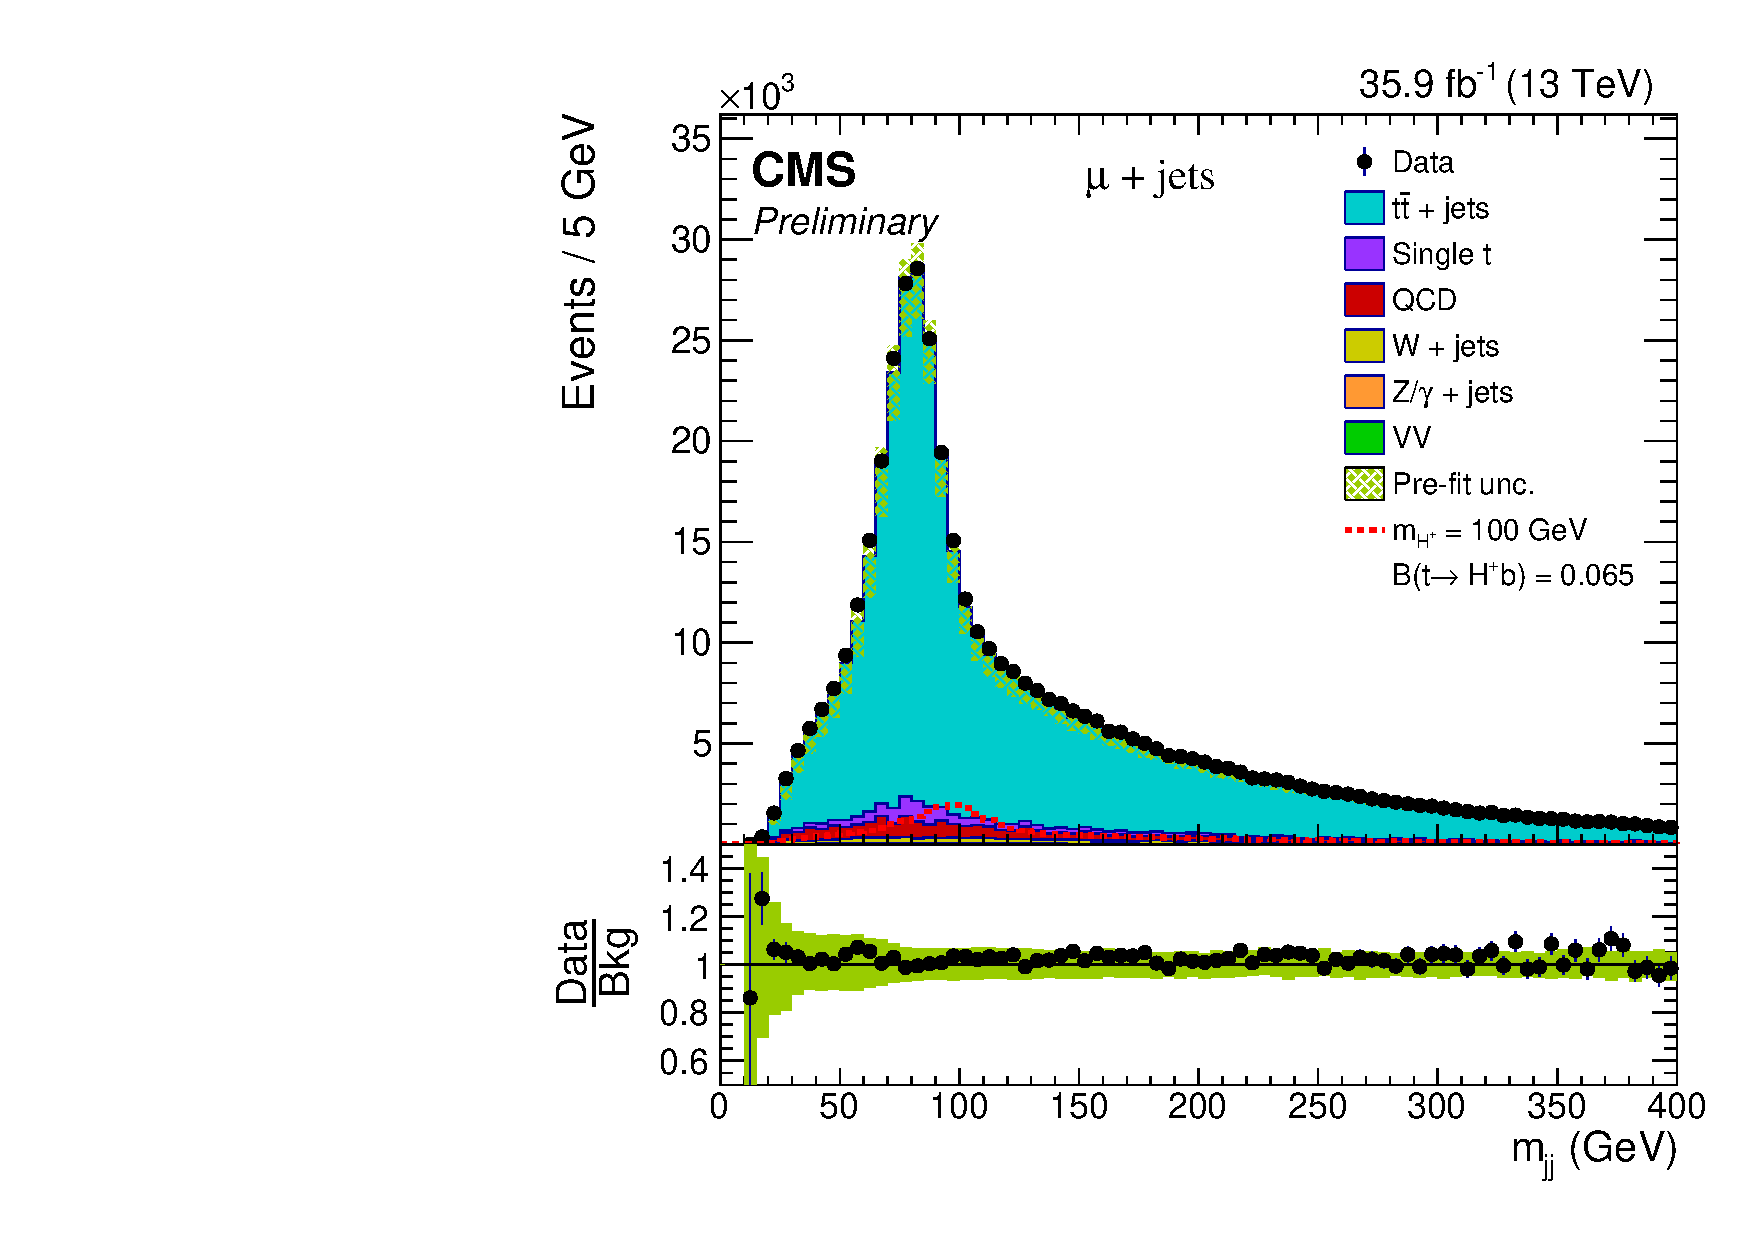
\includegraphics[width=0.49\textwidth]{Image/mjj_muBTag.pdf}
    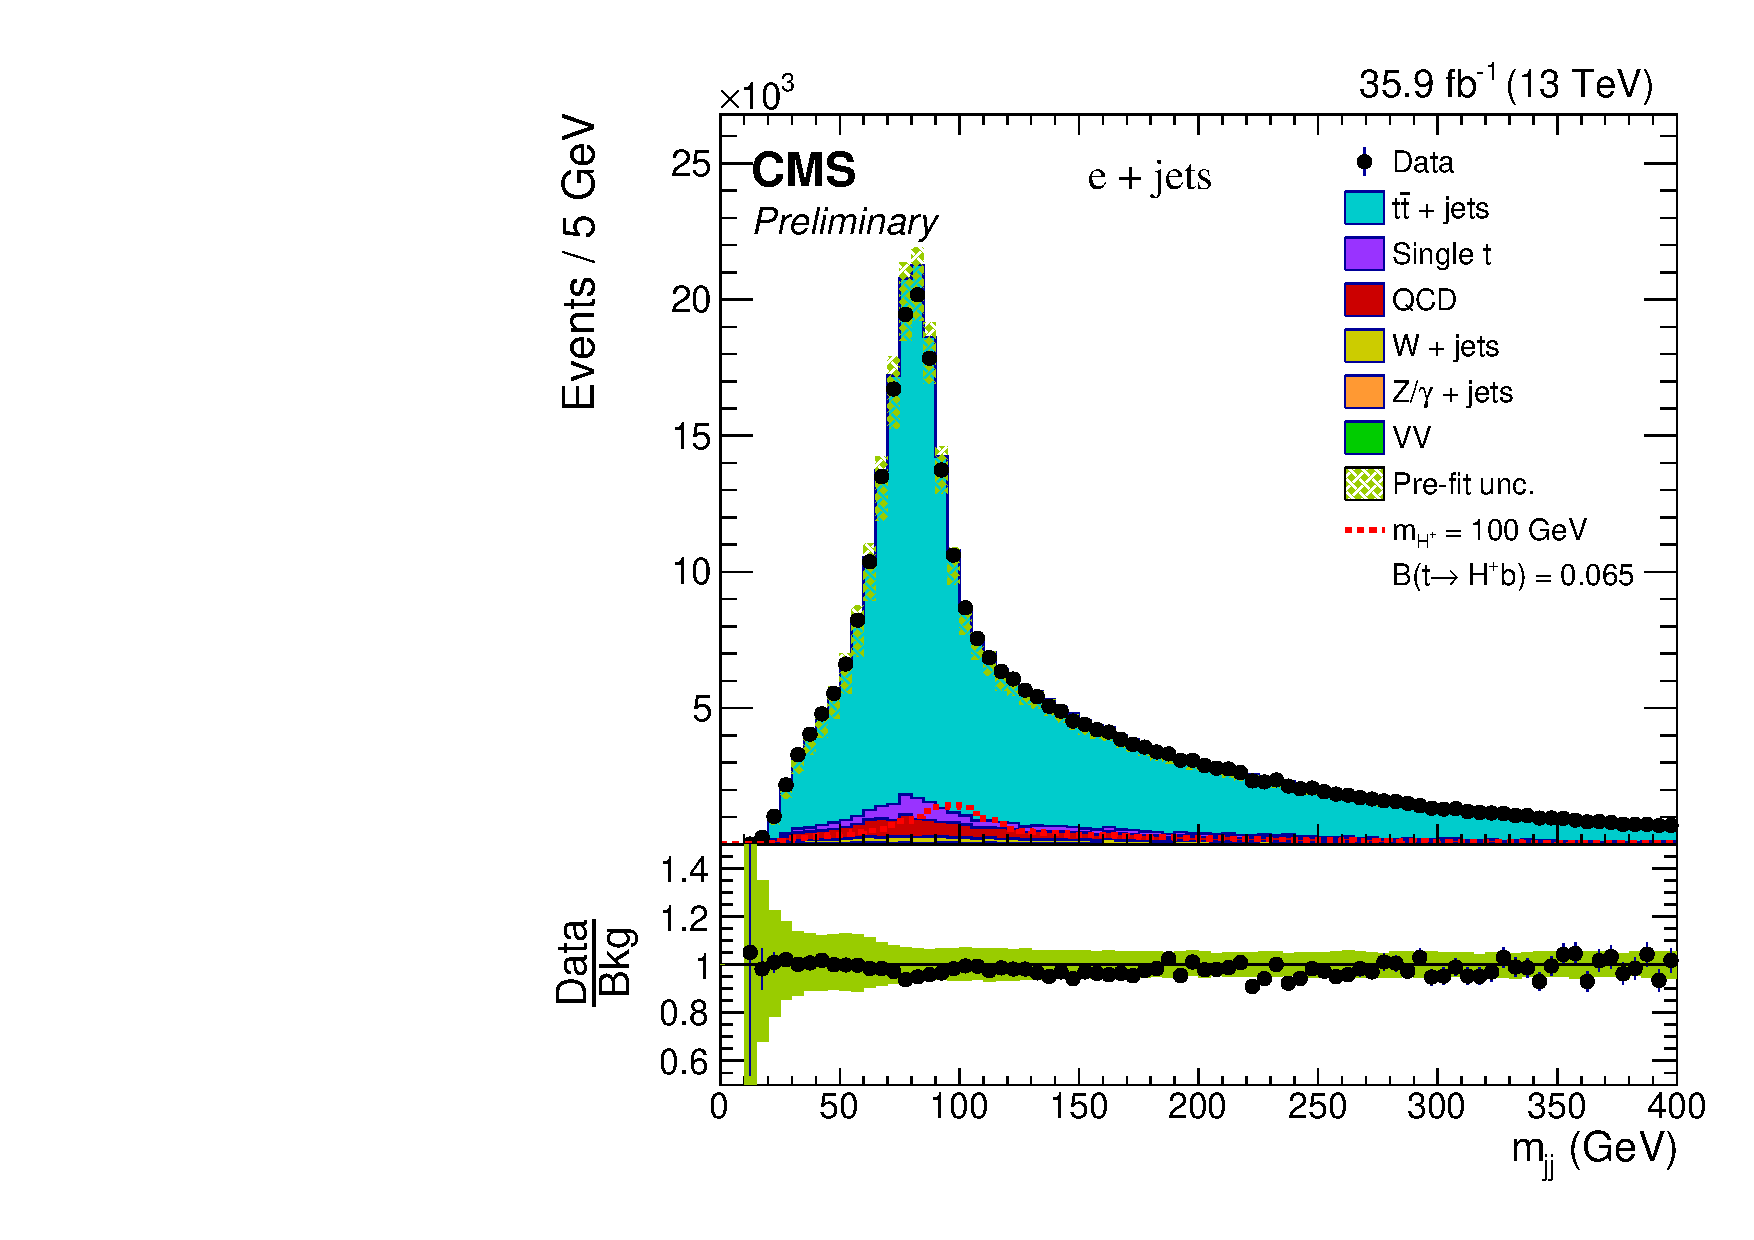
\includegraphics[width=0.49\textwidth]{Image/mjj_eleBTag.pdf}
    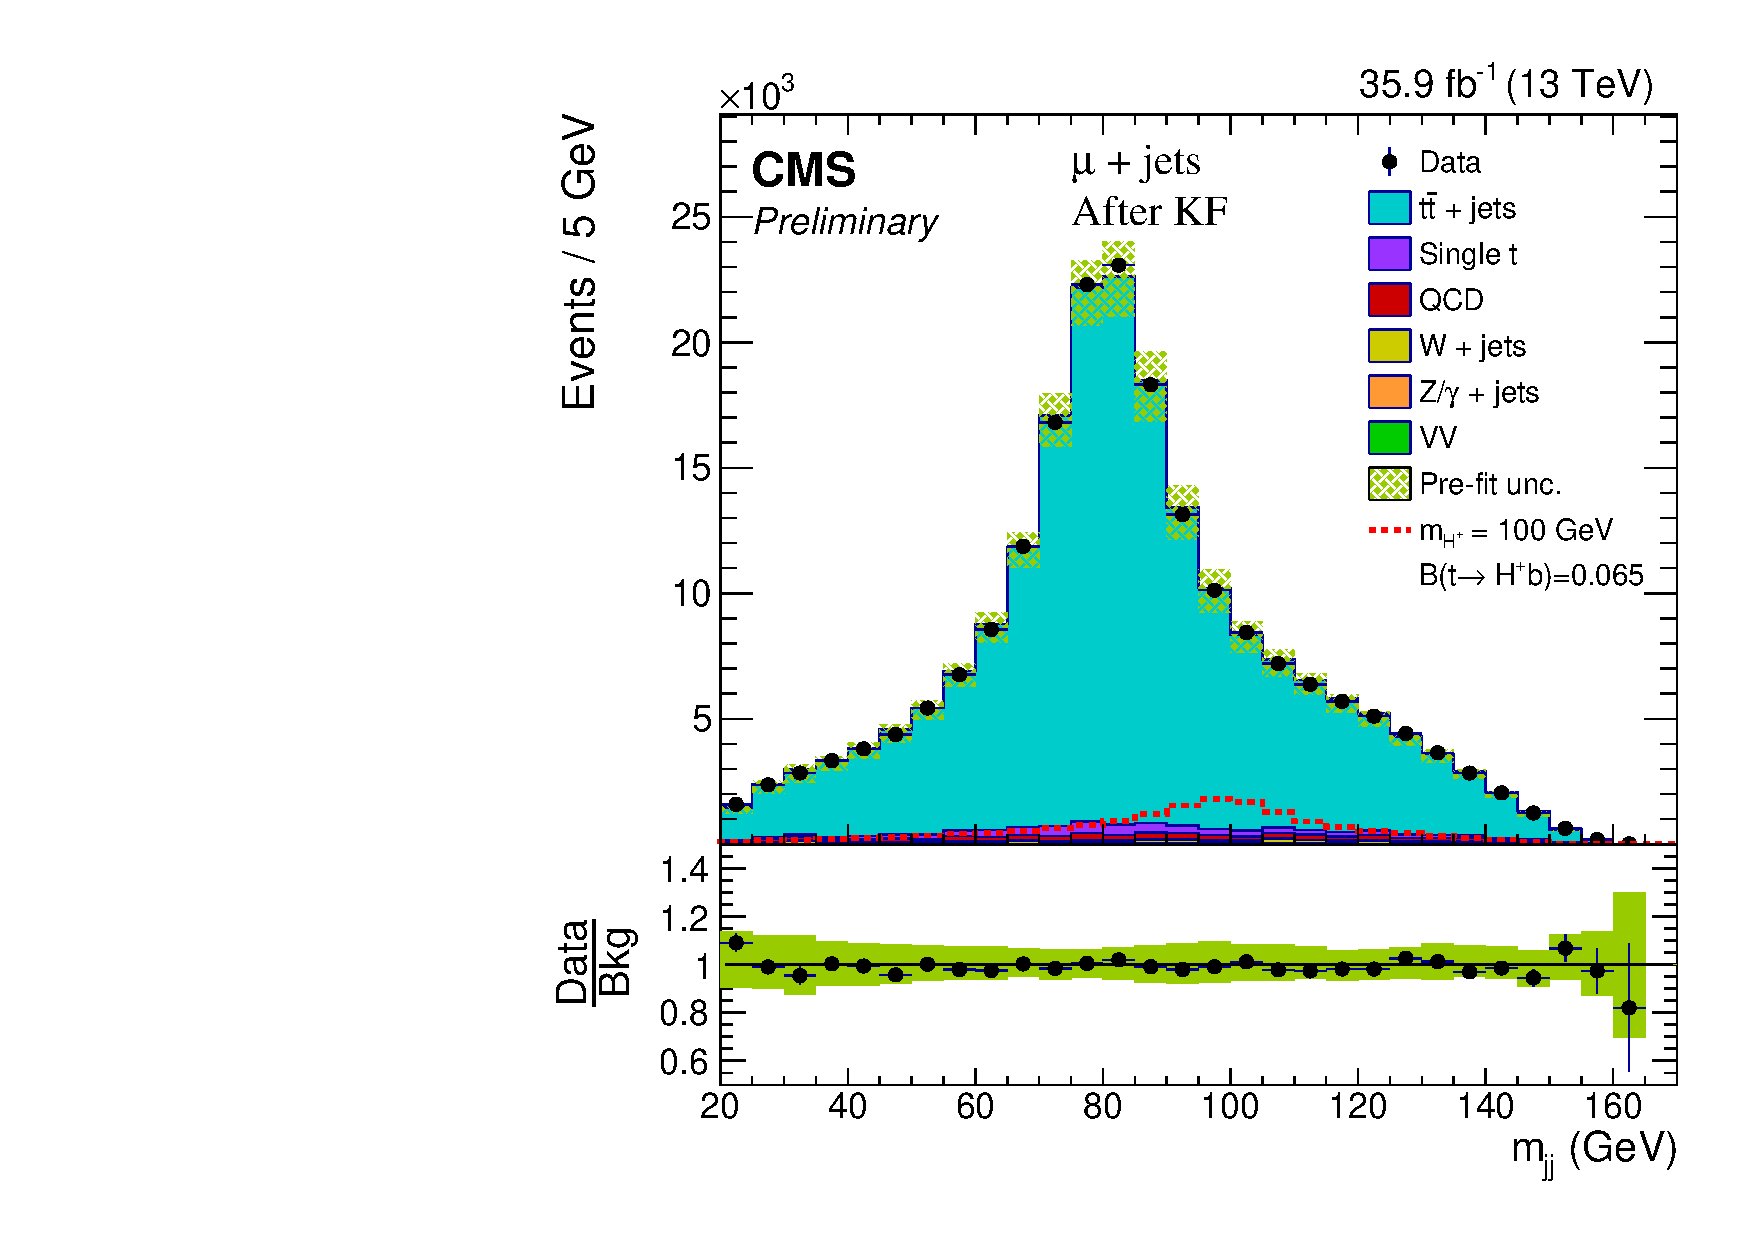
\includegraphics[width=0.49\textwidth]{Image/mjj_kfit_muKinFit.pdf}
    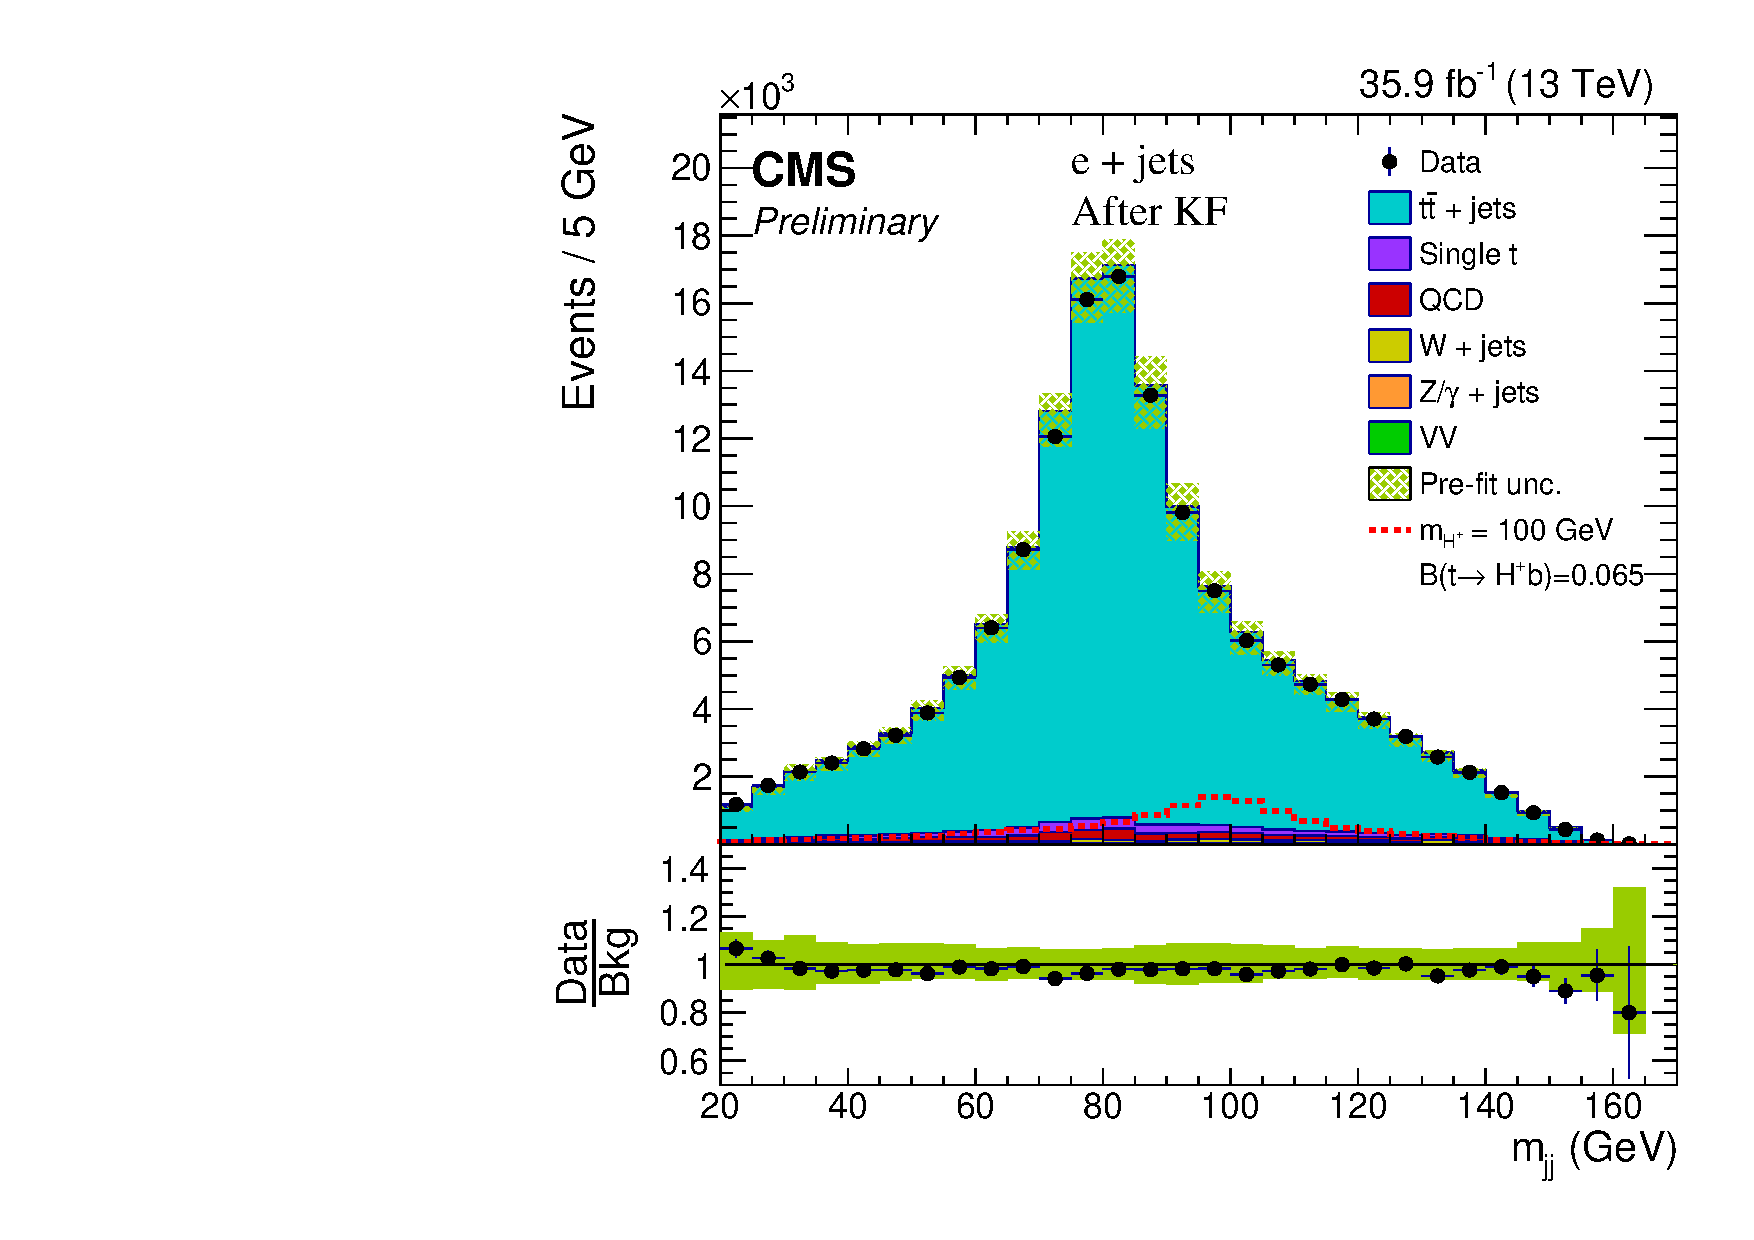
\includegraphics[width=0.49\textwidth]{Image/mjj_kfit_eleKinFit.pdf}
    \caption{Distributions of \mjj, prior to the fit to data, of the two highest \pt light jets for the muon+jets
     channel (left column) and the electron+jets channel (right column). The two distributions in the top row
     are obtained using reconstructed jets. On the other hand, the distributions in the bottom row are calculated using
     kinematic fitted jets after the kinematic fit selection.  The mean of the invariant mass distribution from
     the kinematic fitted jets is closer to the \PW mass as compared to that of reconstructed
 jets. The uncertainty band includes statistical as well as systematic uncertainties.}
    \label{fig:mjjBTagKinFit}
\end{figure}

To select true semileptonic \ttbar events, a kinematic fit (KF) is performed on the
reconstructed objects using the top kinematic fitter package~\cite{DHondt:926540}.
The top kinematic fitter takes physics objects such as leptons, jets, \ptmiss, and their
resolutions as input, and gives improved four-vectors of leptons, jets, and a
neutrino with associated $\chi^2$ and probability of the fit as output. The $x$
and $y$ components of the neutrino momentum are taken from \ptmiss, as the missing transverse
momentum is attributed to the neutrino, and the $z$ component of the neutrino momentum,
$p_z^{\PGn}$, is determined from the fit. The following kinematic constraints are imposed on the semileptonic
\ttbar system:
\begin{linenomath}
\begin{subequations}
\begin{eqnarray}
	m_{\text{inv}}(\PQb_{\text{had}}\PQq\PAQq) = m_{\PQt} = 172.5\GeV \label{eq:constraintKF1}\\
	m_{\text{inv}}(\PQb_{\text{lep}}\ell\PGn_\ell) = m_{\PAQt} = 172.5\GeV \label{eq:constraintKF2}
\end{eqnarray}
\label{eq:constraintKF}
\end{subequations}
\end{linenomath}
After the fit, $p_z^{\PGn}$ is determined from Eq.~\ref{eq:constraintKF2}.
For every event, a $\chi^2$ is constructed and minimized by varying the \pt, $\eta$,
and $\phi$ of each object within their resolution. The values of \pt, $\eta$, and
$\phi$ are finally selected that minimise the $\chi^2$ and at the same time
satisfy Eq.~\ref{eq:constraintKF}. In the output, the top kinematic fitter
gives exactly four jets (two \PQb jets, one from each of the leptonic and hadronic
\PQt decays, and two light jets from the hadronic \PQt decay), a lepton, and a
neutrino. The two light jets coming from the hadronic \PQt decay are further used
for charm tagging. Events for which the fit does not converge are discarded.
Also, the same requirements as for the reconstructed objects are
applied to the kinematically fitted objects. The directions of the kinematically
fitted jets and lepton are required to be compatible with those of the
reconstructed jets and lepton ($\Delta R < 0.2$), respectively.

Further, events are divided exclusively into loose, medium, and tight categories,
based on whether at least one of the light jets passes the loose but neither
passes the medium, at least one passes the medium but neither passes the tight,
or at least one passes the tight working points of the charm tagging selection
requirements~\cite{CMS-PAS-BTV-16-001}, respectively. The \mjj distributions for the exclusive charm
categories are shown in Fig.~\ref{fig:mjj_cTagEx} after a background-only fit to the data. From
these figures, it can be seen that the expected signal to background ratio is
different in the various charm categories, so partitioning the events into
categories results in an improvement in the upper limits on
$\mathcal{B}(\PQt \to \PSHp\PQb)$. The
expected event yields with statistical and systematic (as discussed in Section
\ref{s:secSys}) uncertainties for the different charm categories are shown in
Table~\ref{tab:eventYield}.
\begin{figure}
\centering
{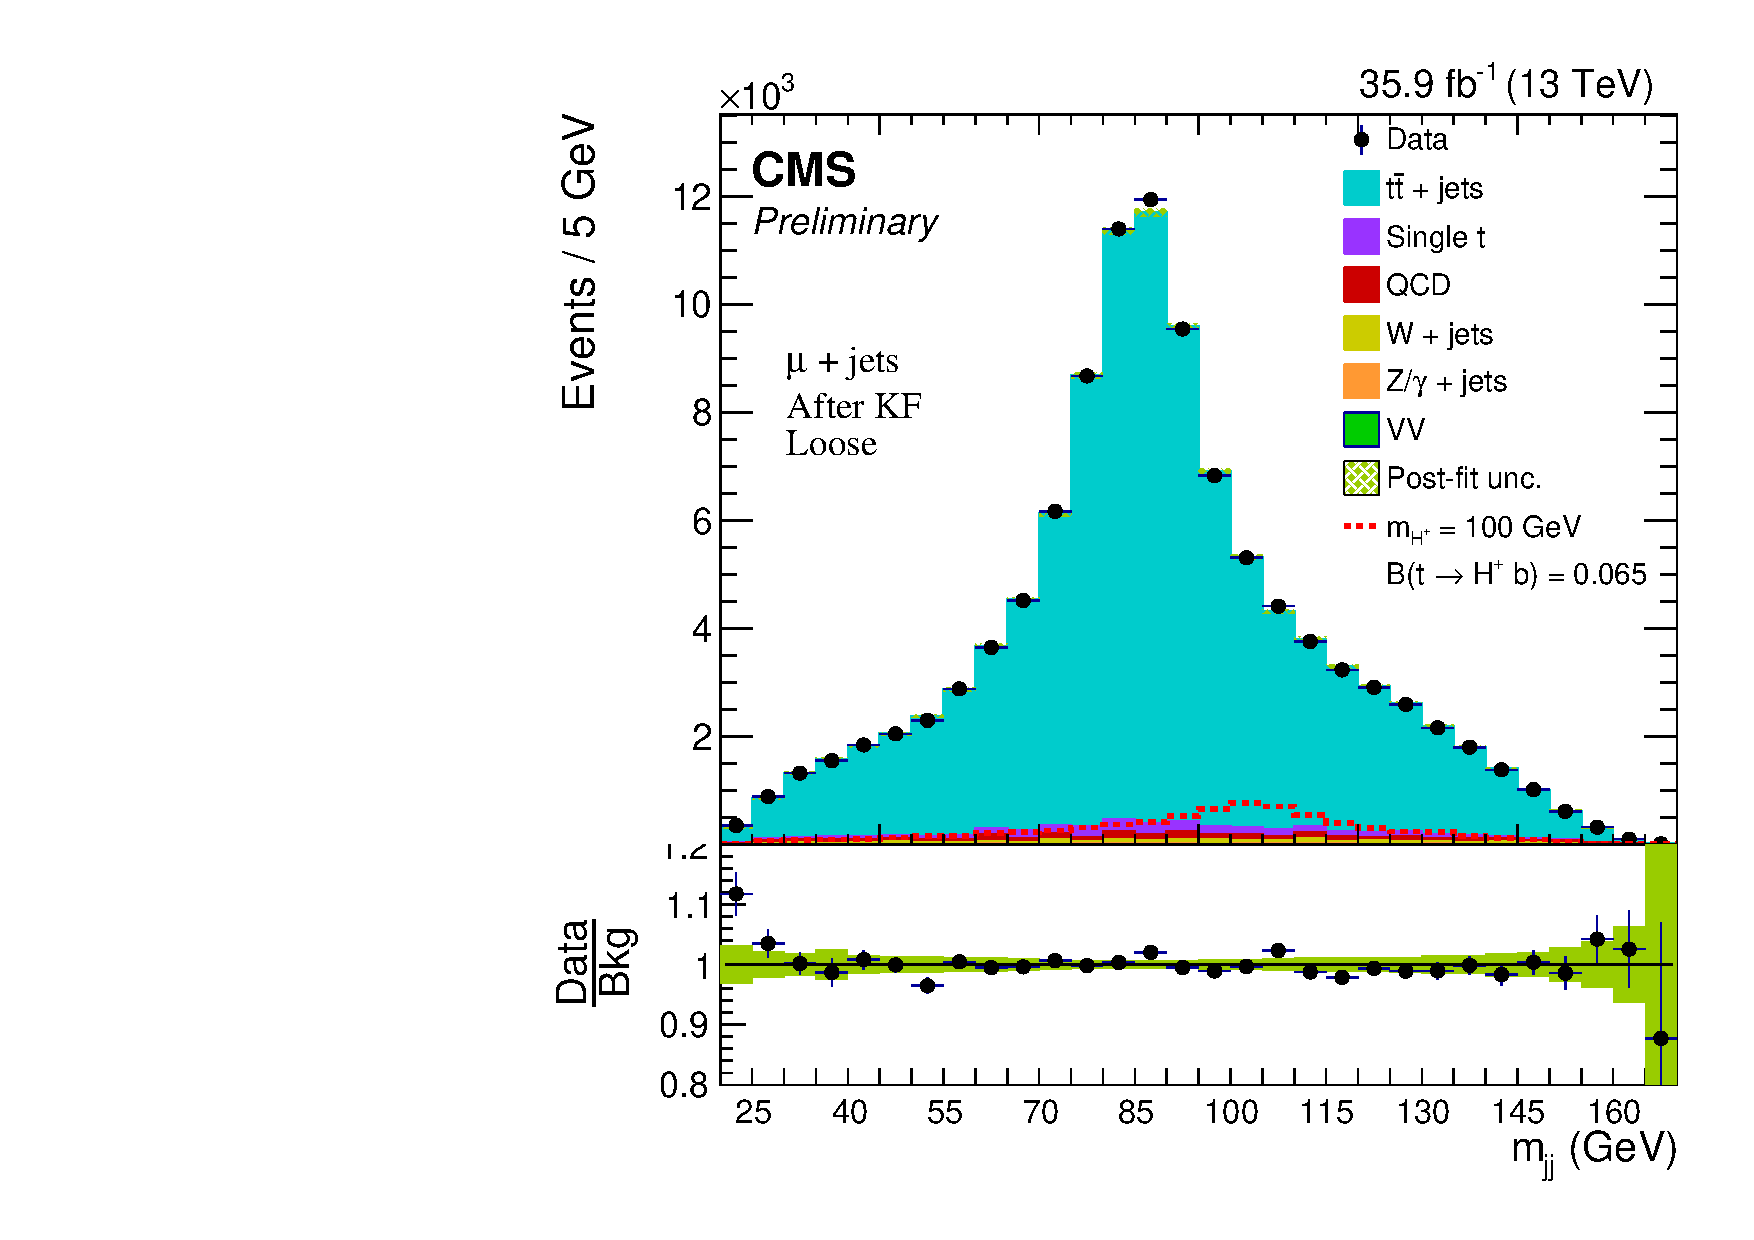
\includegraphics[width=0.45\textwidth]{Image/mjj_postfit_ch1.pdf}}
{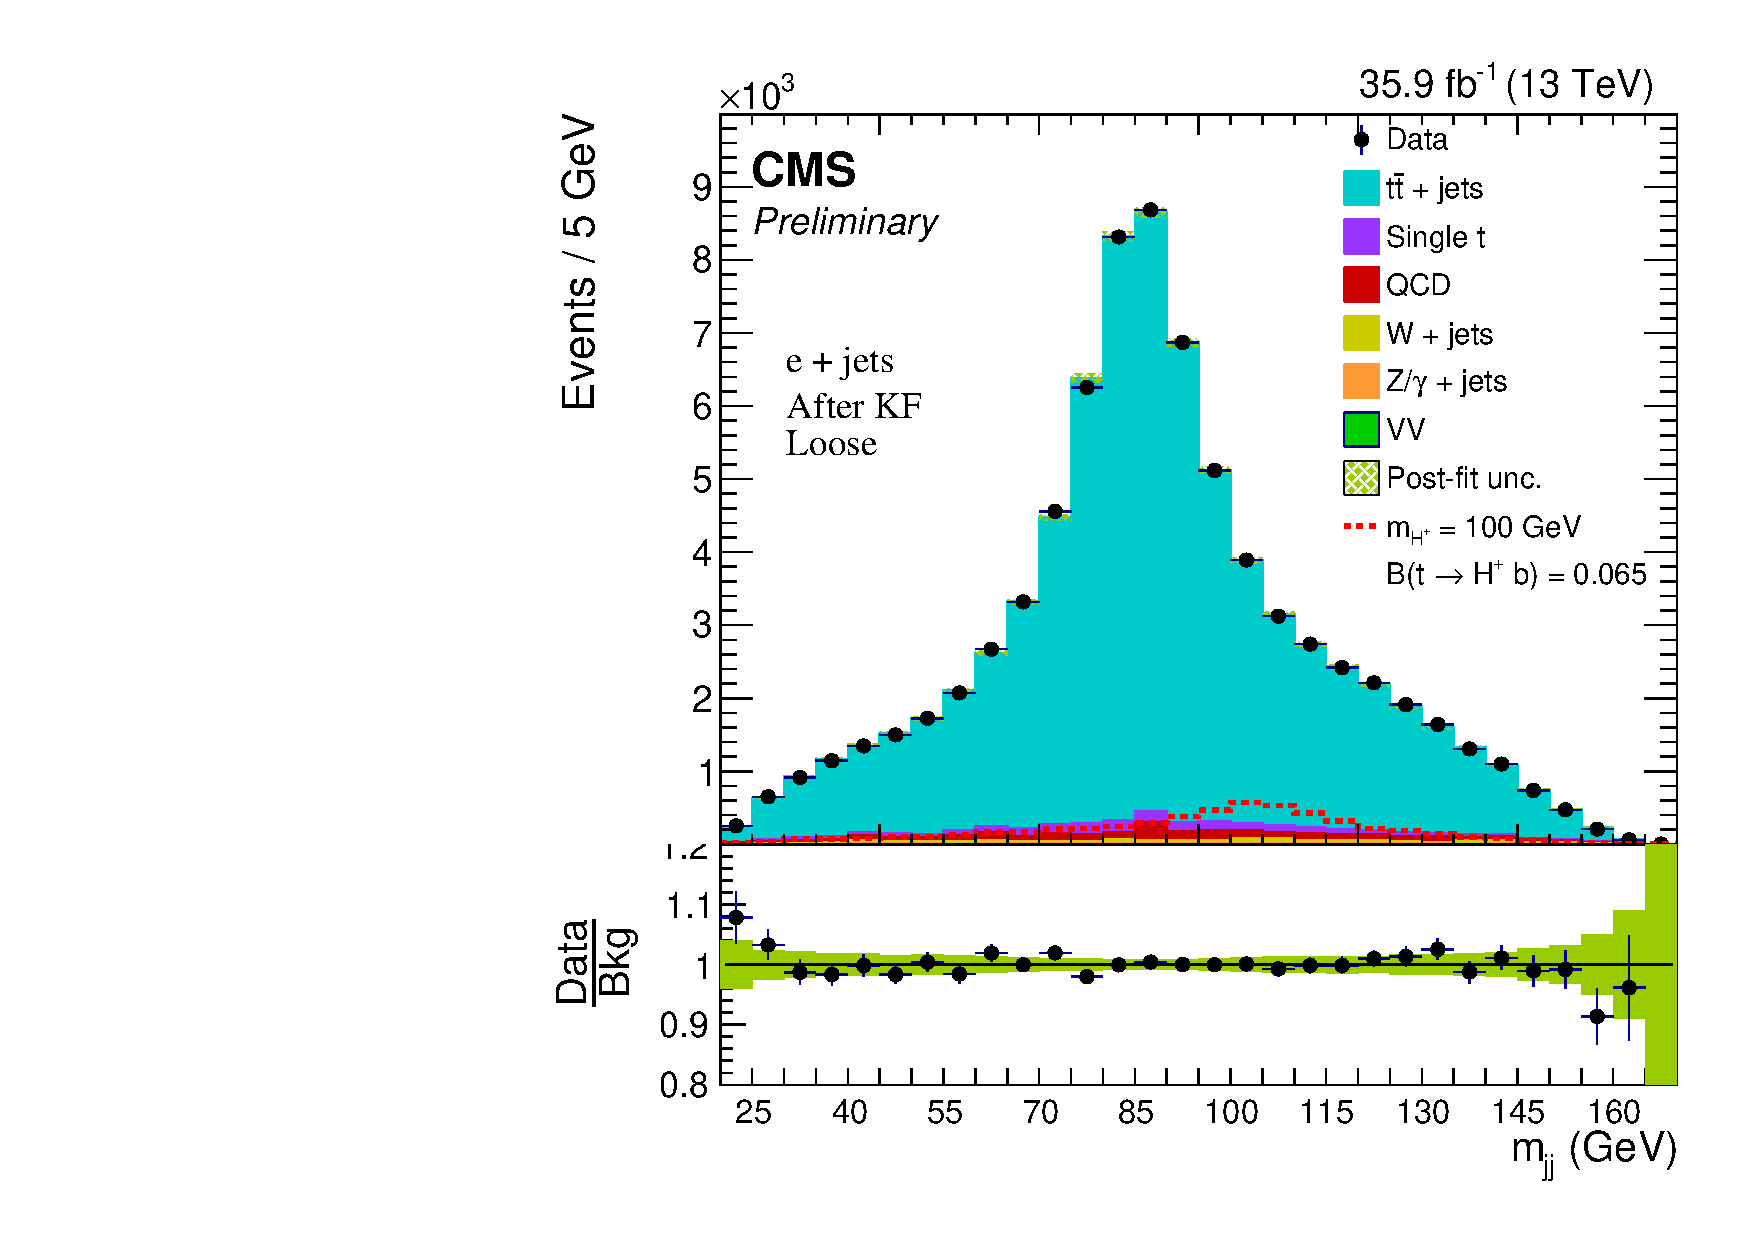
\includegraphics[width=0.45\textwidth]{Image/mjj_postfit_ch4.pdf}}
{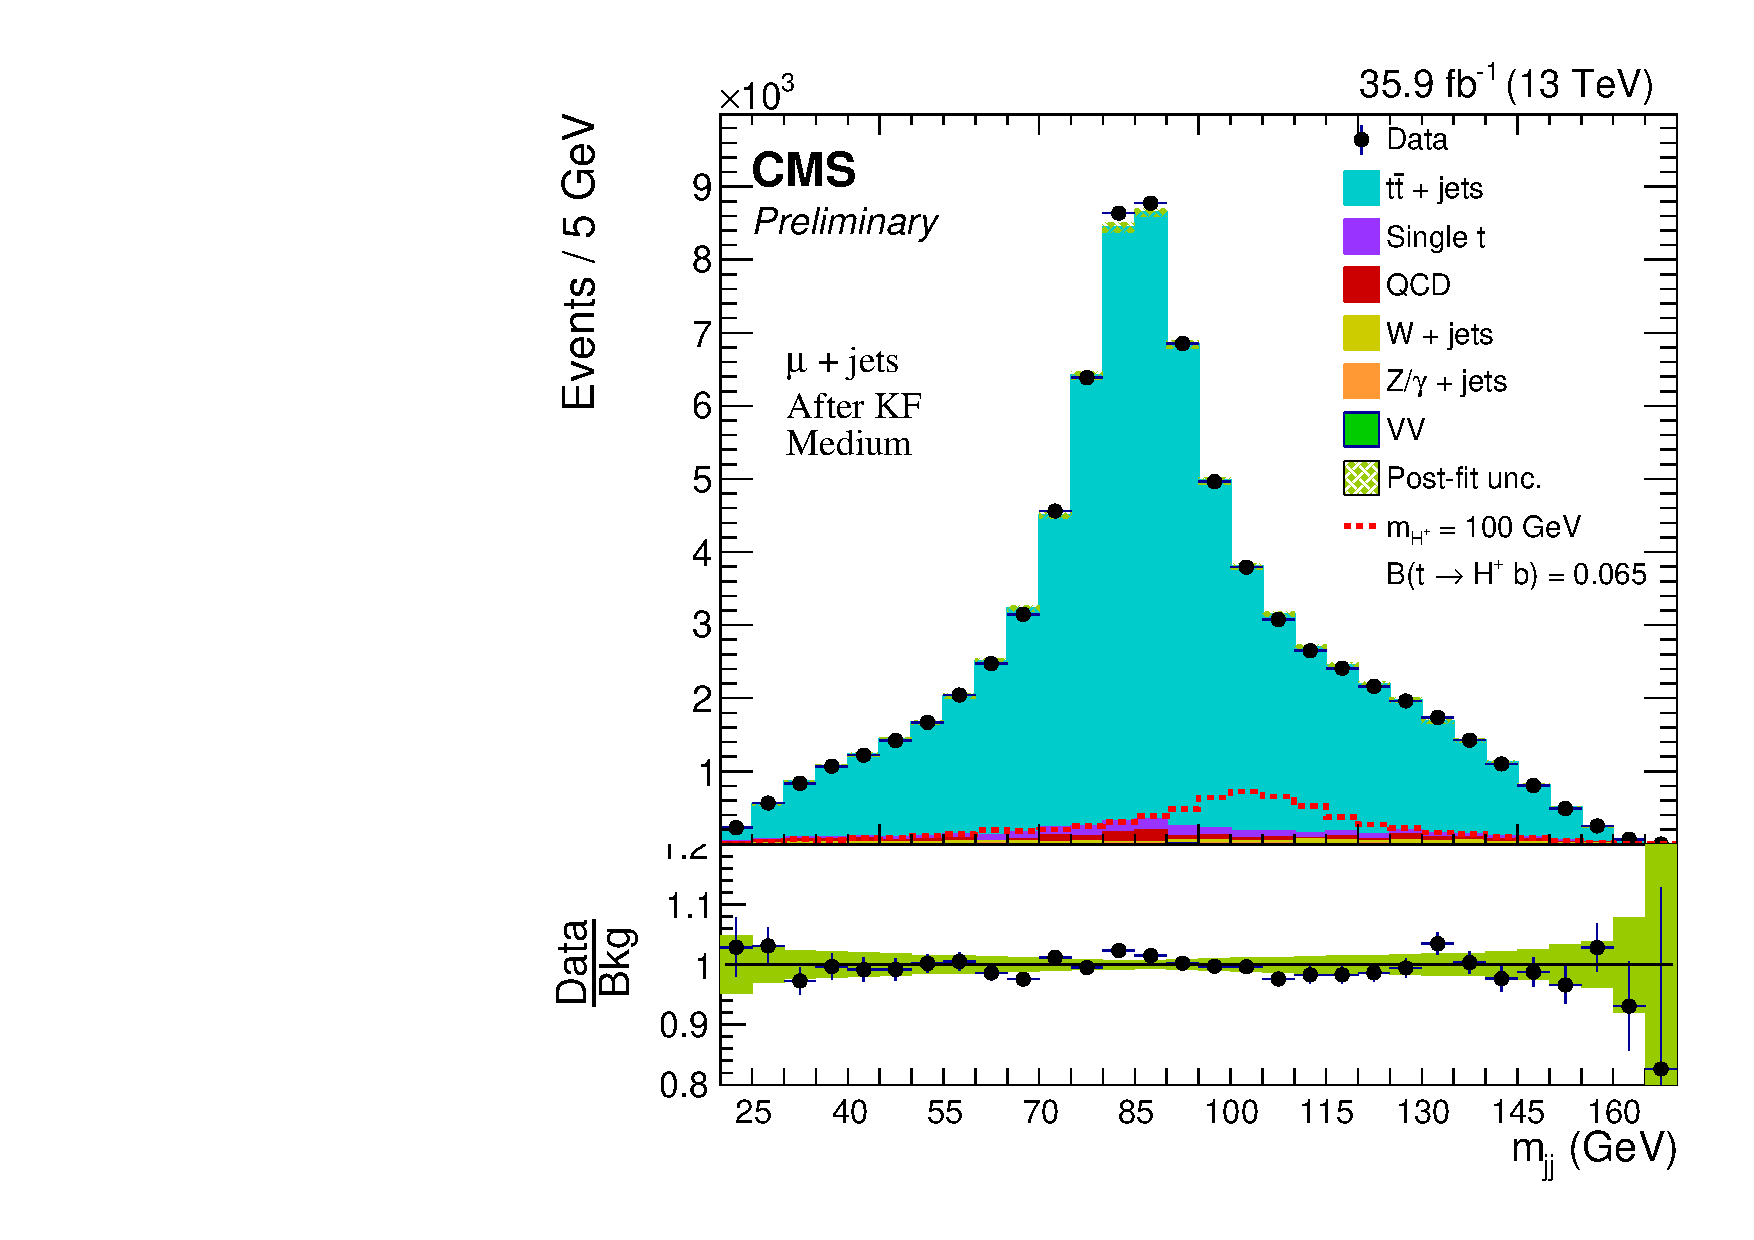
\includegraphics[width=0.45\textwidth]{Image/mjj_postfit_ch2.pdf}}
{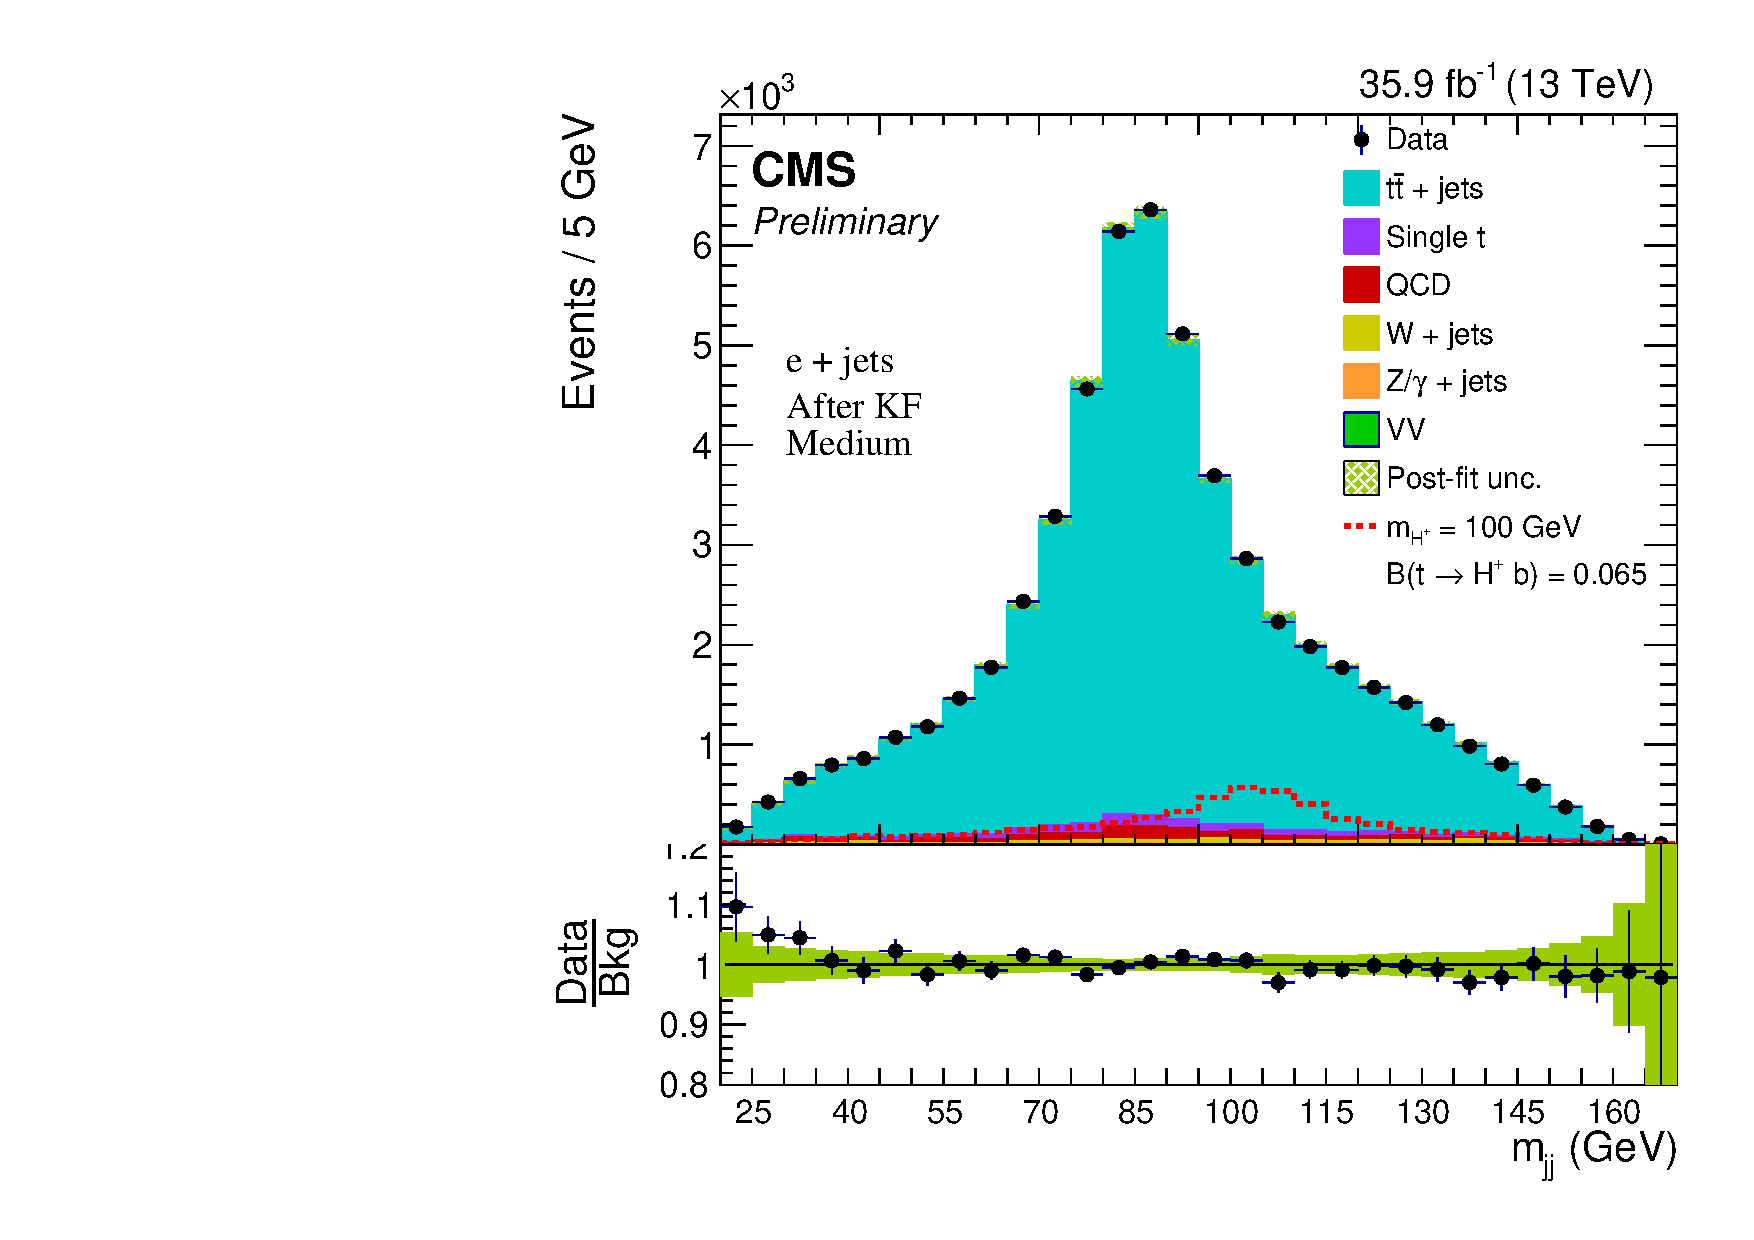
\includegraphics[width=0.45\textwidth]{Image/mjj_postfit_ch5.pdf}}
{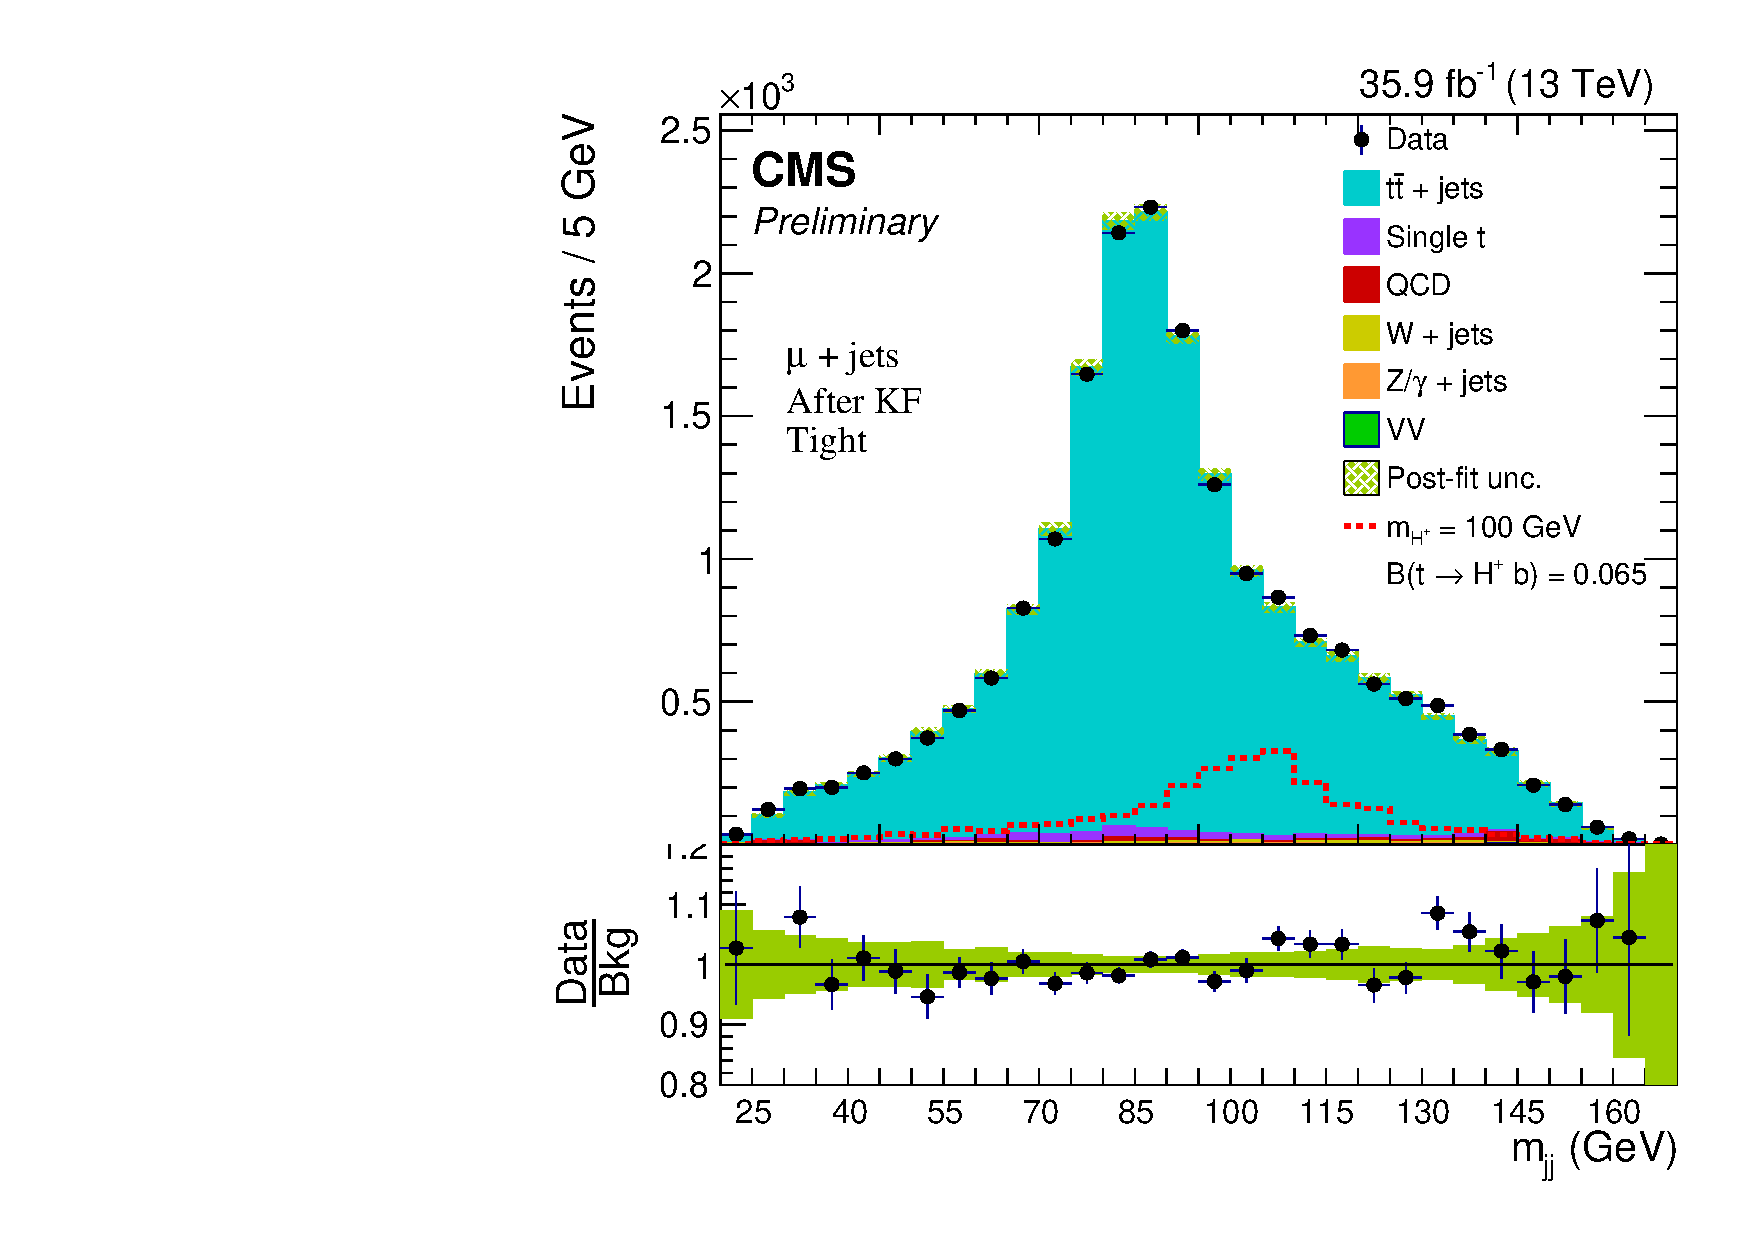
\includegraphics[width=0.45\textwidth]{Image/mjj_postfit_ch3.pdf}}
{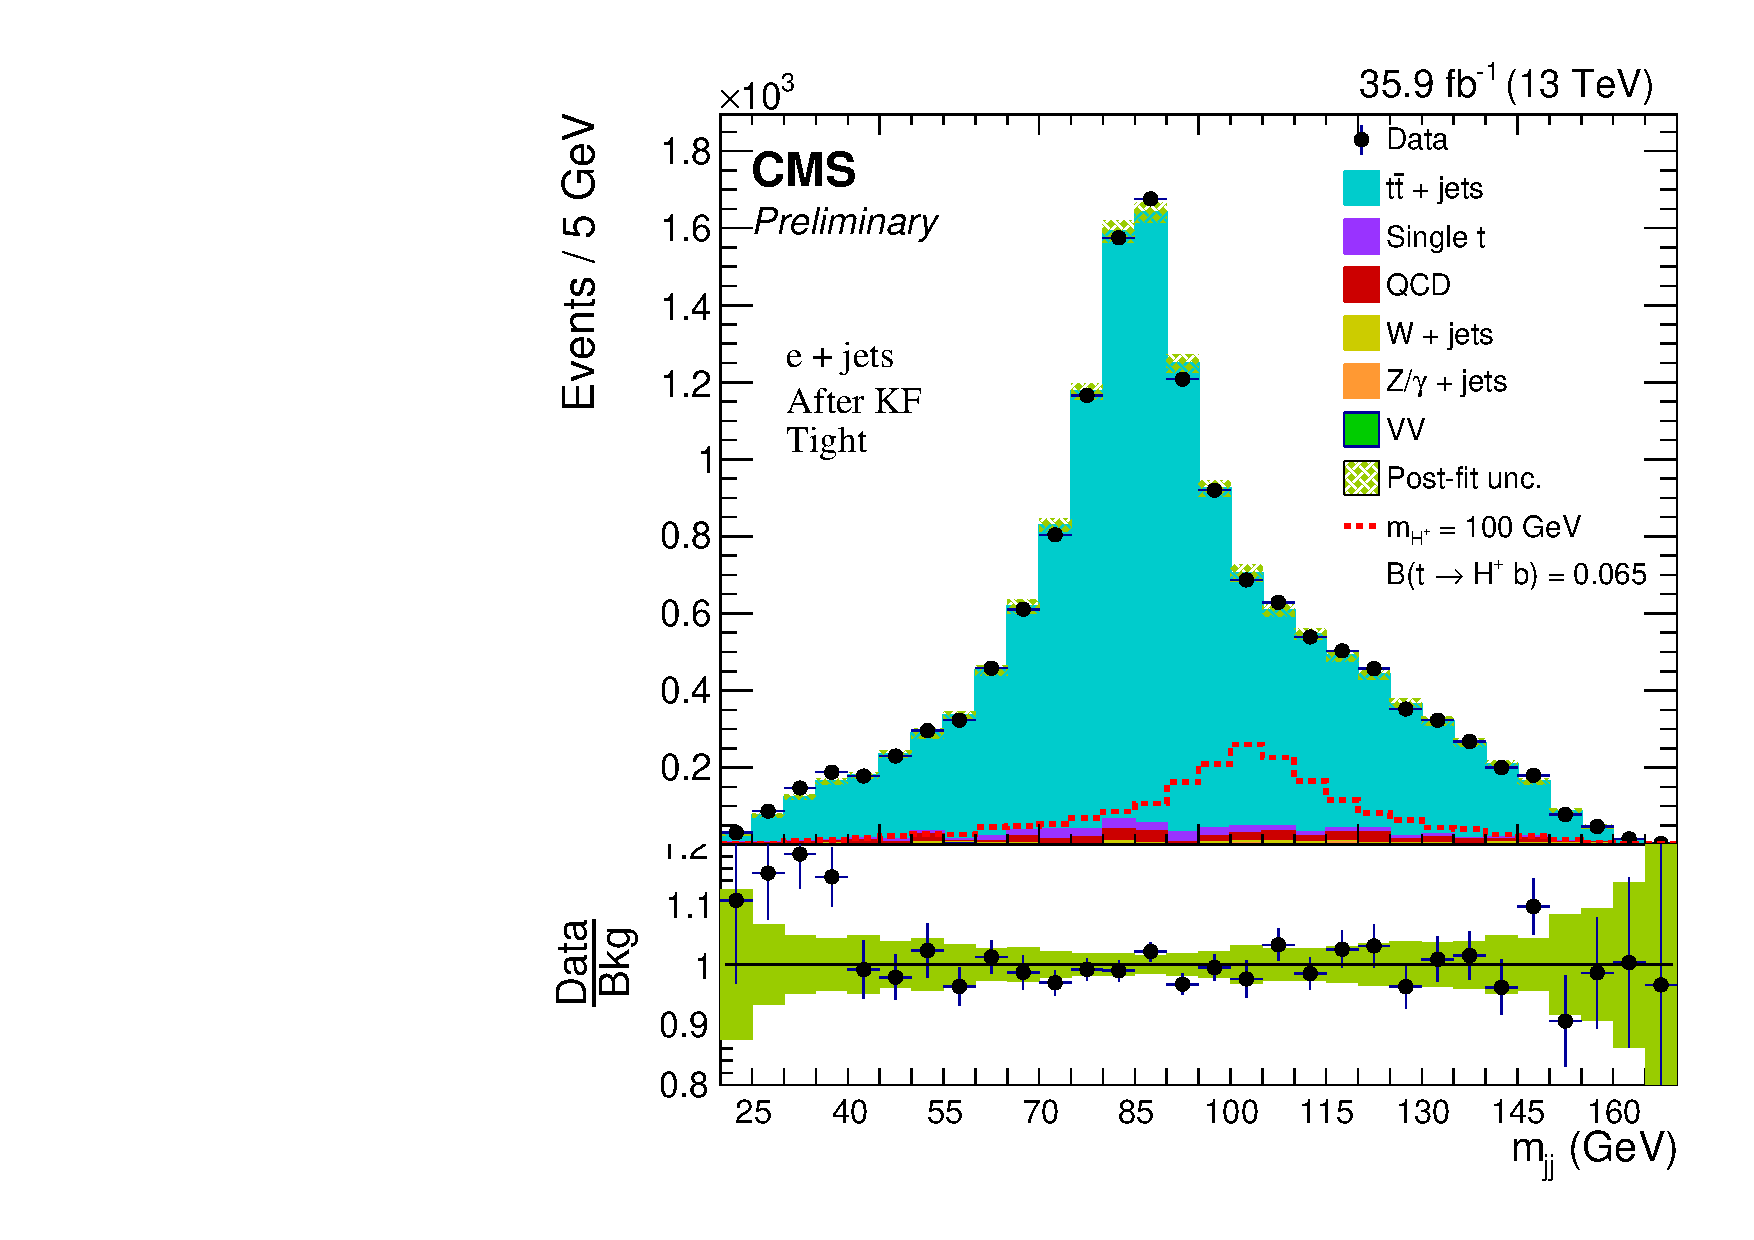
\includegraphics[width=0.45\textwidth]{Image/mjj_postfit_ch6.pdf}}
\caption{Distributions of \mjj, after a background-only fit to the data,
    in the exclusive charm
    categories for the muon + jets (left column) and electron + jets (right
    column) channels. The upper row shows the exclusive loose category, the middle
    row shows the exclusive medium category, and the lower row shows the exclusive
    tight category. The expected signal significance (prior to the fit) can be
    observed to vary across the different categories. The uncertainty band includes
    statistical as well as systematic uncertainties after the background-only fit.}
\label{fig:mjj_cTagEx}
\end{figure}

\begin{table}[ht]
  \centering
\caption{Expected event yields for different signal mass scenarios and backgrounds
    in each of the channels and event categories. The number of events, along with
    the uncertainty (including statistical and systematic effects), is shown. The
    yields for background processes are obtained after a background-only fit to
    the data. The total uncertainty on the background process is calculated
    by taking into account all the positive as well as negative
    correlations among the fit parameters.}
\label{tab:eventYield}
  \cmsTable{
\begin{tabular}{cccccccc}
\hline
\hline
\multicolumn{1}{c}{{\bf{Process}}} & \multicolumn{2}{c}{{Loose}} & \multicolumn{2}{c}{{Medium}} & \multicolumn{2}{c}{{Tight}} \\
                  & $\mu$ + jets   &  e + jets      & $\mu$ + jets   &  e + jets      & $\mu$ + jets   &  e + jets \\
\hline
\hline
$m_{\PSHp}=80$ \GeV & 7171 $\pm$ 682 & 5375 $\pm$ 503 & 6137 $\pm$ 556 & 4683 $\pm$ 440 & 2471 $\pm$ 282 & 1826 $\pm$ 206\\
$m_{\PSHp}=90$ \GeV & 7171 $\pm$ 722 & 5556 $\pm$ 539 & 6300 $\pm$ 607 & 4818 $\pm$ 472 & 2442 $\pm$ 277 & 1843 $\pm$ 211\\
$m_{\PSHp}=100$ \GeV & 7382 $\pm$ 722 & 5480 $\pm$ 523 & 6591 $\pm$ 642 & 4911 $\pm$ 418 & 2570 $\pm$ 293 & 1967 $\pm$ 221\\
$m_{\PSHp}=120$ \GeV & 7073 $\pm$ 692 & 5291 $\pm$ 528 & 6378 $\pm$ 606 & 4732 $\pm$ 415 & 2466 $\pm$ 265 & 1923 $\pm$ 217\\
$m_{\PSHp}=140$ \GeV & 5716 $\pm$ 628 & 4338 $\pm$ 442 & 5043 $\pm$ 511 & 3816 $\pm$ 405 & 1869 $\pm$ 212 & 1472 $\pm$ 170\\
$m_{\PSHp}=150$ \GeV & 4218 $\pm$ 480 & 3215 $\pm$ 367 & 3584 $\pm$ 407 & 2774 $\pm$ 320 & 1233 $\pm$ 157 & 1015 $\pm$ 138\\
$m_{\PSHp}=155$ \GeV & 3447 $\pm$ 419 & 2522 $\pm$ 336 & 2758 $\pm$ 361 & 2205 $\pm$ 296 & 935 $\pm$ 152 & 762 $\pm$ 101\\
$m_{\PSHp}=160$ \GeV & 2593 $\pm$ 318 & 2053 $\pm$ 252 & 2210 $\pm$ 299 & 1699 $\pm$ 246 & 682 $\pm$ 108 & 506 $\pm$ 68\\
\hline
SM $\ttbar$ + jets & 99130 $\pm$ 458 & 71874 $\pm$ 498 & 72481 $\pm$ 354 & 52470 $\pm$ 329 & 18624 $\pm$ 136 & 13397 $\pm$ 134 \\
Single \PQt & 2618 $\pm$ 212 & 1918 $\pm$ 165 & 1865 $\pm$ 150 & 1357 $\pm$ 114 & 421 $\pm$ 35 & 304 $\pm$ 27 \\
QCD multijet & 2207 $\pm$ 301 & 2153 $\pm$ 481 & 1385 $\pm$ 214 & 1426 $\pm$ 255 & 232 $\pm$ 50 & 364 $\pm$ 61 \\
\PW + jets & 1260 $\pm$ 146 & 1008 $\pm$ 92 & 872 $\pm$ 114 & 649 $\pm$ 57 & 112 $\pm$ 17 & 83 $\pm$ 14 \\
$\PZ/\PGg$ + jets & 167 $\pm$ 21 & 220 $\pm$ 26 & 118 $\pm$ 15 & 126 $\pm$ 15 & 51 $\pm$ 7 & 30 $\pm$ 3 \\
VV & 62 $\pm$ 6 & 43 $\pm$ 6 & 47 $\pm$ 11 & 11 $\pm$ 4 & 11 $\pm$ 3 & 4 $\pm$ 1 \\
\hline
All background & 105444 $\pm$ 606 & 77216 $\pm$ 719 & 76768 $\pm$ 455 & 56039 $\pm$ 436 & 19451 $\pm$ 151 & 14182 $\pm$ 151 \\
\hline
Data & 105485 & 77244 & 76811 & 56051 & 19451 & 14179 \\
\hline
\end{tabular}
}
\end{table}


%%%%%%%%% SYSTEMATICS %%%%%%%%%%%%%%%%%%%%%%%%%%
\section{Systematic uncertainties}
\label{s:secSys}
There are various sources of systematic uncertainty which may arise due to detector calibration effects,
uncertainty in the measured reconstructed efficiency, the theoretical modeling of signal events, and other
effects.

The uncertainty in the integrated luminosity is 2.5\% for 2016 data taking~\cite{CMS-PAS-LUM-17-001}. To
account for uncertainty in the total inelastic cross section of 69.2\unit{mb}, this is varied by its
uncertainty of 4.7\% and the simulated events are reweighted to match the resulting pileup distributions. The
lepton reconstruction efficiency is different in data and simulated samples; to correct for this, lepton scale
factors are applied to the simulated events. The systematic uncertainty in the lepton scale factor is
3.0\%~\cite{Sirunyan:2018fpa,Khachatryan:2015hwa}. The \pt of jets in the simulated samples are corrected
using the jet energy scale (JES) and jet energy resolution (JER) scale factors. The jet energy correction is
also propagated to correct \ptmiss. The systematic uncertainties due to JES and JER on the \pt of the jets and \ptmiss are
considered by varying these scale factors within their uncertainties.  The \PQb and \PQc tagging efficiencies
are different in simulation and data, and scale factors are applied to the simulated events. To estimate the
corresponding systematic uncertainty, the \PQb and \PQc tag scale factors are varied within their
uncertainties, with proper correlations applied.  To estimate the systematic uncertainty on the data-driven
QCD multijet background estimation, the muon (electron) relative isolation selection value is conservatively
changed to 0.17 (0.11) and the corresponding changes in the QCD yields are determined.
To account for the statistical uncertainty, in each bin of \mjj, one shape nuisance
parameter is considered for all background and charged Higgs samples.

Each distribution for simulated events is normalized to the expected number of events in data, using the
factor $L_\text{data}\sigma_\text{sim}/N_\text{sim}$, where $L_\text{data}$ is the integrated luminosity in the
data sample, $N_\text{sim}$ is the total number of events in the simulated sample, and $\sigma_\text{sim}$ is
the cross section for the simulated process considered; the uncertainties in $\sigma_\text{sim}$ thus
contribute to the uncertainty in each background prediction. It is found that the
\pt distribution of \PQt quarks in \ttbar events in data is softer compared to that from simulated
samples~\cite{Khachatryan:2016mnb}. This is corrected by applying the following weight as a
function of \pt for SM \ttjets and charged Higgs samples:
\begin{linenomath}
\begin{equation}
w_\text{top}=\sqrt{\text{SF}(\PQt)\text{SF}(\PAQt)},\ \text{where}\ \text{SF}\equiv\exp(0.0615 - 0.0005\pt).
\label{eq:top_wt}
\end{equation}
\end{linenomath}
The values in the exponent are given in Ref.~\cite{Khachatryan:2016mnb}.
The generator-level $\pt$ of the \PQt and \PAQt are used to calculate
SF. To evaluate the systematic uncertainty in $w_\text{top}$, it is varied to 1 and $w_\text{top}^2$.
The SM \ttjets sample was generated with \mt = 172.5\GeV. To evaluate the effect of the chosen \mt on the \mjj
distribution, alternate \ttjets samples with \mt = 171.5 and 173.5\GeV are considered.
In the simulated samples, the NLO matrix element parton shower matching is varied by the damping parameter $h_\text{damp}$.
Additional SM $\ttjets$ samples are generated by varying $h_\text{damp}$ up and down and are used to observe the effect of
$h_\text{damp}$. Similarly, SM $\ttjets$ samples where the renormalization and factorisation scales have been
varied up and down are used to evaluate the uncertainties due to these scales.

All the systematic and statistical uncertainties are shown in Table~\ref{tab:sysUnc}.
Among all systematics, the uncertainties on the data-driven QCD multijet background, lepton
selection, \ttjets cross section, jet energy scale, and \PQb/\PQc tagging have a significant
impact on the expected limit. The expected limit changes by 4.7\%, 2.7\%, 2.7\%,
1.3\%, and 0.7\%, respectively, for the corresponding uncertainties. The
effect of each of the remaining systematic uncertainties on the expected limit
is estimated to be less than 0.3\%.

\begin{table}[ht]
  \centering
\caption{Systematic and statistical uncertainties in \%, prior to the fit to data, for the exclusive charm categories in the muon (electron) channel. The "---" indicates that the corresponding uncertainties are not considered for the given process.}
\label{tab:sysUnc}
  \cmsTable{
\begin{tabular}{cccccccc}
\hline
\hline
Category &Process& Pileup & jet \& \ptmiss & \PQb \& \PQc-jet & Normalization& Statistical & top \pt\\
\hline
\hline
 Loose  & $m_{\PSHp}=100$ \GeV &  0.81 (1.2) & 7.4 (6.8) &  6.3 (6.4) & 6.1 (6.1) & 1 (1.2) & 0.49 (1) \\
 & \ttjets &  0.97 (1.2) & 6.9 (6.9) &  5.9 (5.8) & 6.1 (6.1) & 0.19 (0.22) & 0.73 (1.3) \\
 & Single \PQt  &  1.1 (0.82) & 9.1 (10) &  6.8 (6.7) & 5 (5) & 1 (1.2) & --- \\
 & \PW + jets &  1.4 (1.1) & 18 (13) &  14 (9.7) & 5 (5) & 6.8 (4.6) & --- \\
 & $\PZ/\PGg$ + jets &  0.4 (2.3) & 20 (18) &  11 (9.3) & 4.5 (4.5) & 5.9 (4.4) & --- \\
 & VV &  4.5 (11) & 8.7 (16) &  10 (12) & 4 (4) & 21 (22) & --- \\
 & QCD multijet &  --- & --- &  --- & 13 (23) & 7.9 (7.7) & --- \\
\hline
 Medium & $m_{\PSHp}=100$ \GeV &  0.65 (0.36) & 6.7 (4.8) &  6.9 (6.7) & 6.1 (6.1) & 1.1 (1.3) & 0.65 (1.5) \\
 & \ttjets &  0.25 (0.45) & 6.2 (6.2) &  7.4 (7.3) & 6.1 (6.1) & 0.23 (0.27) & 0.62 (1.4) \\
 & Single \PQt  &  0.73 (0.29) & 8.5 (8.6) &  7.9 (8.3) & 5 (5) & 1.3 (1.5) & --- \\
 & \PW + jets &  1.5 (2.5) & 20 (12) &  12 (12) & 5 (5) & 5 (5.8) & --- \\
 & $\PZ/\PGg$ + jets &  1.5 (3.5) & 21 (17) &  12 (12) & 4.5 (4.5) & 6.3 (6) & --- \\
 & VV &  13 (7.2) & 28 (54) &  22 (11) & 4 (4) & 21 (35) & --- \\
 & QCD multijet &  --- & --- &  --- & 15 (16) & 12 (10) & --- \\
\hline
 Tight  & $m_{\PSHp}=100$ \GeV &  1.3 (1.4) & 5.2 (5.6) &  9.9 (9.4) & 6.1 (6.1) & 1.7 (1.9) & 0.85 (1.1) \\
 & \ttjets &  1.3 (0.93) & 5.9 (6) &  10 (9.5) & 6.1 (6.1) & 0.44 (0.5) & 0.47 (1.3) \\
 & Single \PQt  &  0.72 (0.38) & 7.8 (8.9) &  11 (10) & 5 (5) & 2.6 (3) & --- \\
 & \PW + jets &  2.4 (3) & 23 (27) &  19 (13) & 5 (5) & 13 (14) & --- \\
 & $\PZ/\PGg$ + jets & 8.8 (4.6) & 8.6 (13) &  20 (13) & 4.5 (4.5) & 9.5 (15) & --- \\
 & VV &  0.66 (8.9) & 27 (0) &  35 (10) & 4 (4) & 40 (1e+02) & --- \\
 & QCD multijet &  --- & --- &  --- & 11 (13) & 28 (18) & --- \\
\hline
\end{tabular}
}
\end{table}


%%%%%%%%%%%%%%%%%%%%%%%%%% RESULTS %%%%%%%%%%%%%%%%
\section{Results}
\label{s:secResults}
The event yields after all selection requirements have been applied, along with the combined systematic and
statistical uncertainty, are shown in Table~\ref{tab:eventYield} for the muon + jets and electron + jets
channels. From Table~\ref{tab:eventYield}, it can be seen that the total expected background number of events
agrees with the data within the uncertainties.
The absence of a charged Higgs signal in the data is characterized by setting exclusion limits on the
branching ratio $\mathcal{B}(\PQt \to \PSHp\PQb)$, assuming that $\mathcal{B}(\PSHp \to \PQc\PAQs)$ = 100\%.  The
number of signal events in data, $\Delta N$, is determined by subtracting the predicted number of background
events from the total observed number,
assuming that the difference is due to signal events only. The difference $\Delta N$ is calculated using the
following formula:
\begin{linenomath}
\begin{equation}
\Delta N = N^\text{BSM}_{\ttjets} - N^\text{SM}_{\ttjets} = 2x(1-x)N^\text{sig}  +  [(1 - x)^{2} - 1]N^\text{SM}_{\ttjets}.
\label{eq:deltaN}
\end{equation}
\end{linenomath}
where $N^\text{BSM}_{\ttjets}$ is the number of events from beyond the standard model (BSM) decays of $\ttbar$,
including the production of charged Higgs bosons, $N^\text{sig}$ is the number of events from the simulated
signal sample, $N^\text{SM}_{\ttjets }$ is the number of events from SM $\ttjets$ process as shown in
Fig.~\ref{fig:feyn_diag_sig}, and $x$ is the branching ratio of $\PQt \to \PSHp\PQb$. The values of $N^\text{sig}$ and
$N^\text{SM}_{\ttjets}$ are shown in Table~\ref{tab:eventYield} for the muon + jets and electron + jets
channels. The factor 2 in Eq.~\ref{eq:deltaN} is derived from the assumption that the event
yield and $\mathcal{B}(\PAQt \to \PSHm\PAQb)$ for \PSHm are
the same as that of \PSHp and $\mathcal{B}(\PQt \to \PSHp\PQb)$, respectively.
An asymptotic 95\% \CL limit on $\mathcal{B}(\PQt \to \PSHp\PQb)$ is
calculated using the \CLs method~\cite{Read:2002hq,Junk:1999kv} with likelihood
ratios~\cite{Cowan:2010js}. The exclusion limits as a function of charged Higgs mass
using the \mjj distribution from combining different exclusive event categories based on charm tagging are shown in Fig.
\ref{fig:limitPlot} and in Tables \ref{tab:limit_muon_ele} and \ref{tab:limit_lepton}.
Among the individual categories, the expected limits from the exclusive
medium category are best, followed by those from the exclusive loose
and tight categories. By construction, the exclusion
limits on $\mathcal{B}(\PAQt \to \PSHm\PAQb)$ are the same as those on $\mathcal{B}(\PQt \to \PSHp\PQb)$.

\begin{figure}
    \centering
    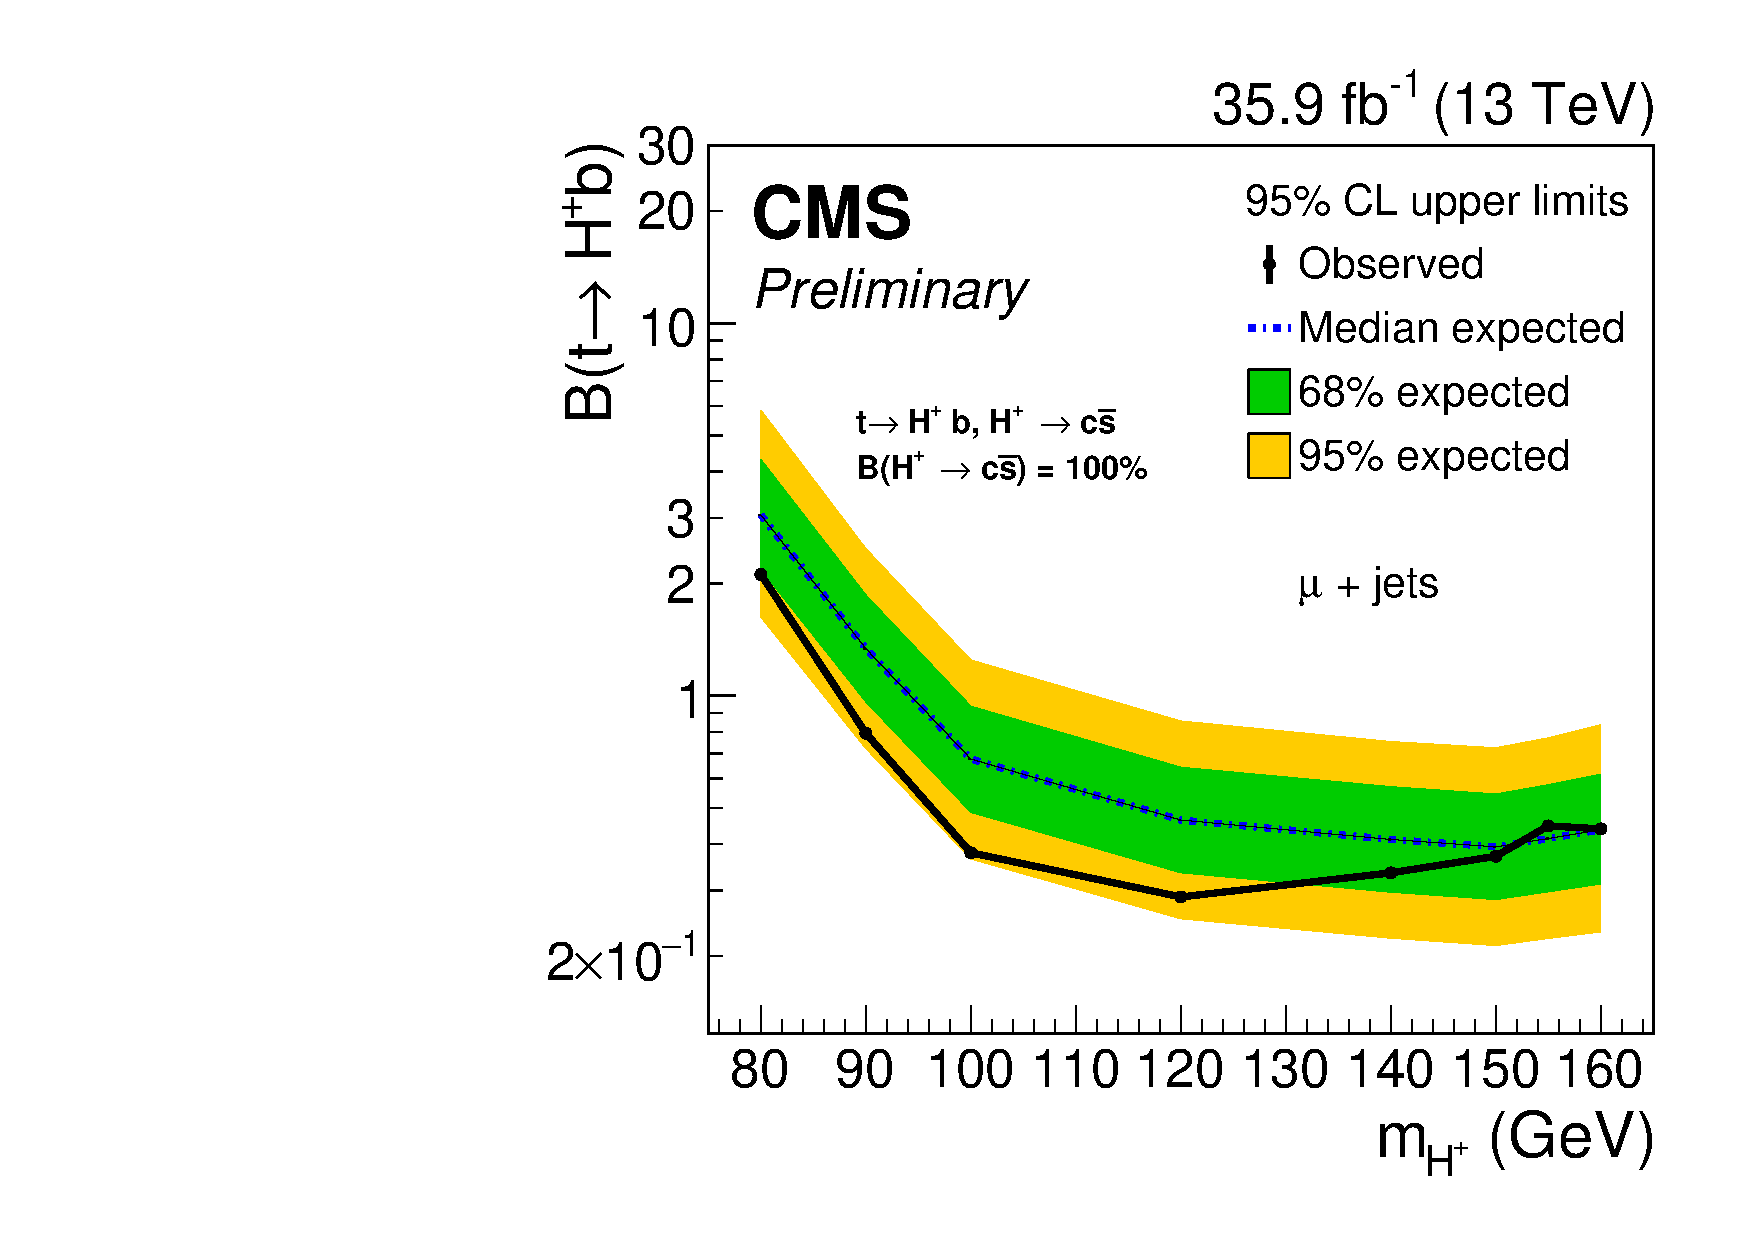
\includegraphics[width=0.45\textwidth]{Image/limit_mu_Cat3_cTagEx.pdf}
    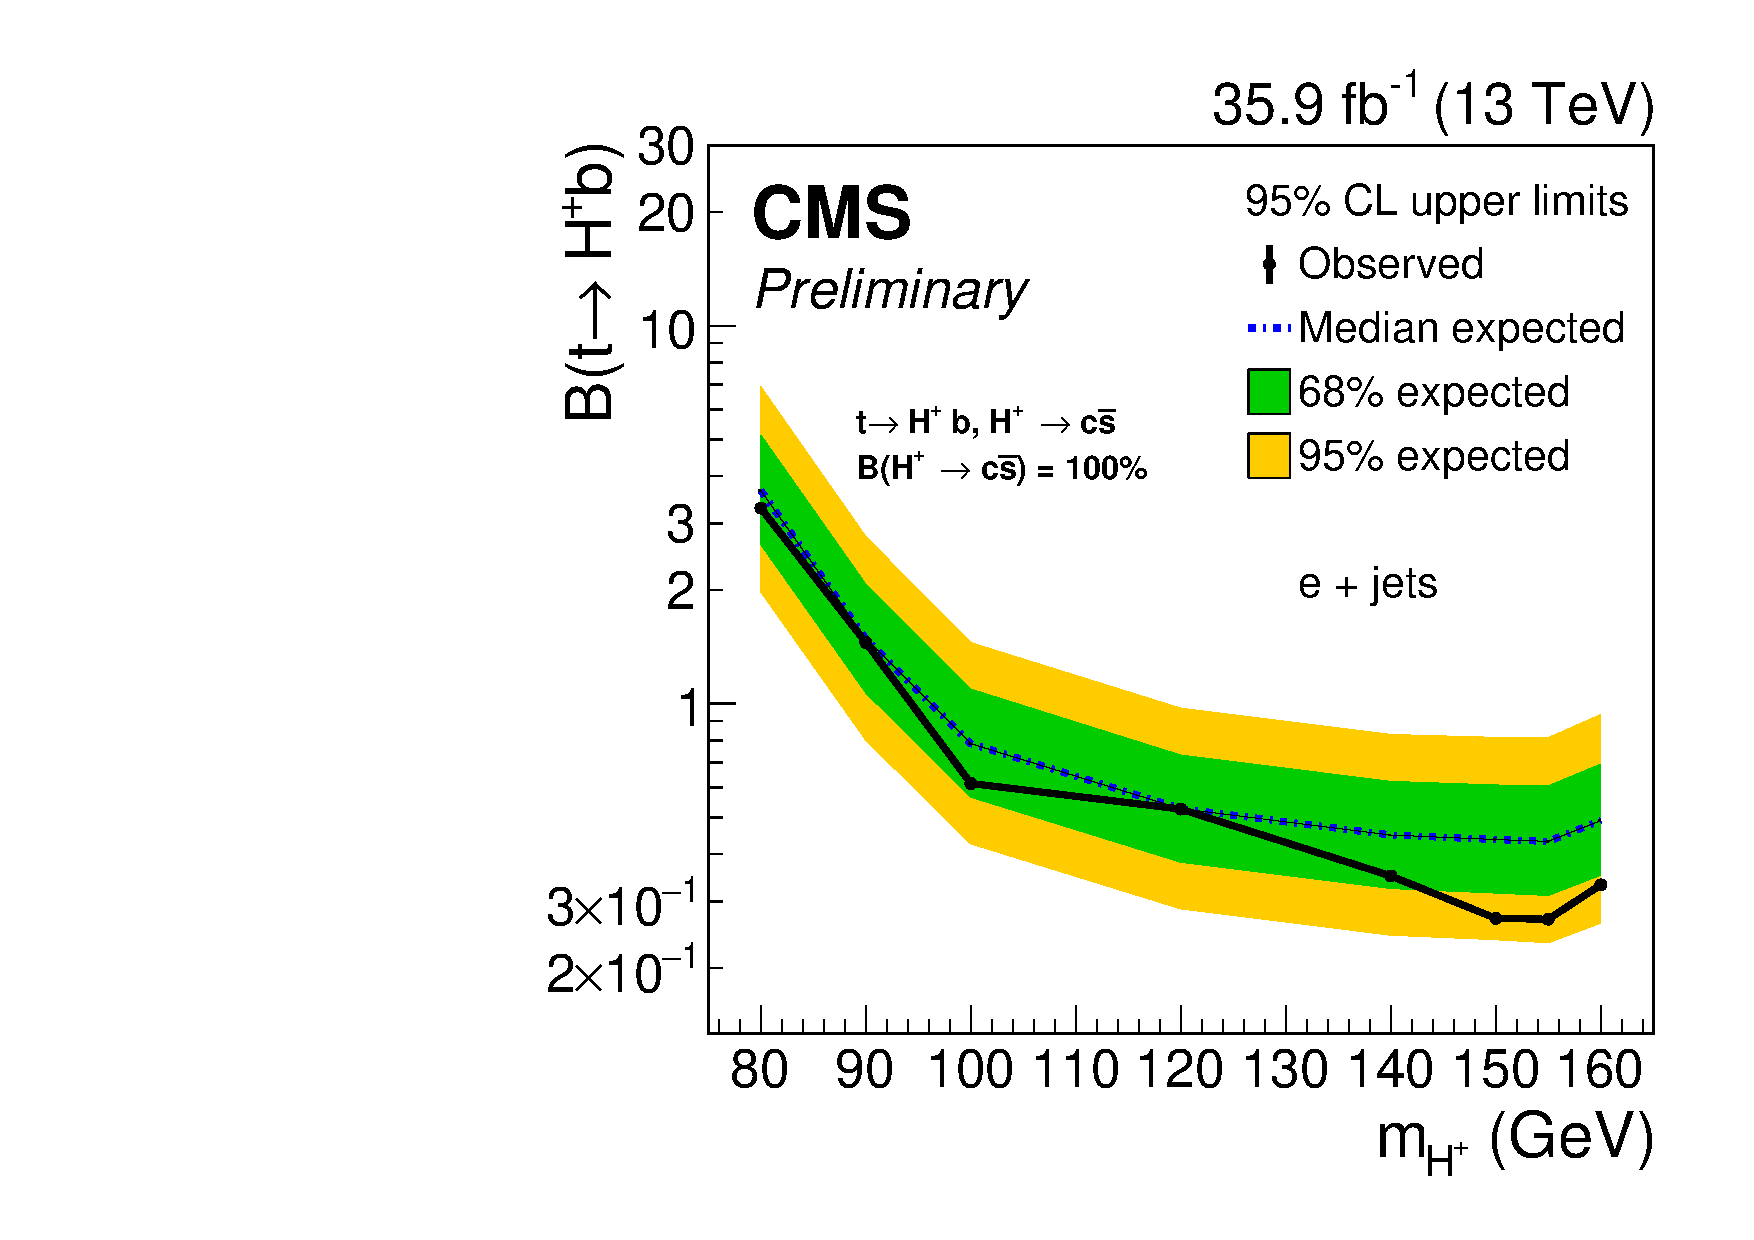
\includegraphics[width=0.45\textwidth]{Image/limit_ele_Cat3_cTagEx.pdf}
    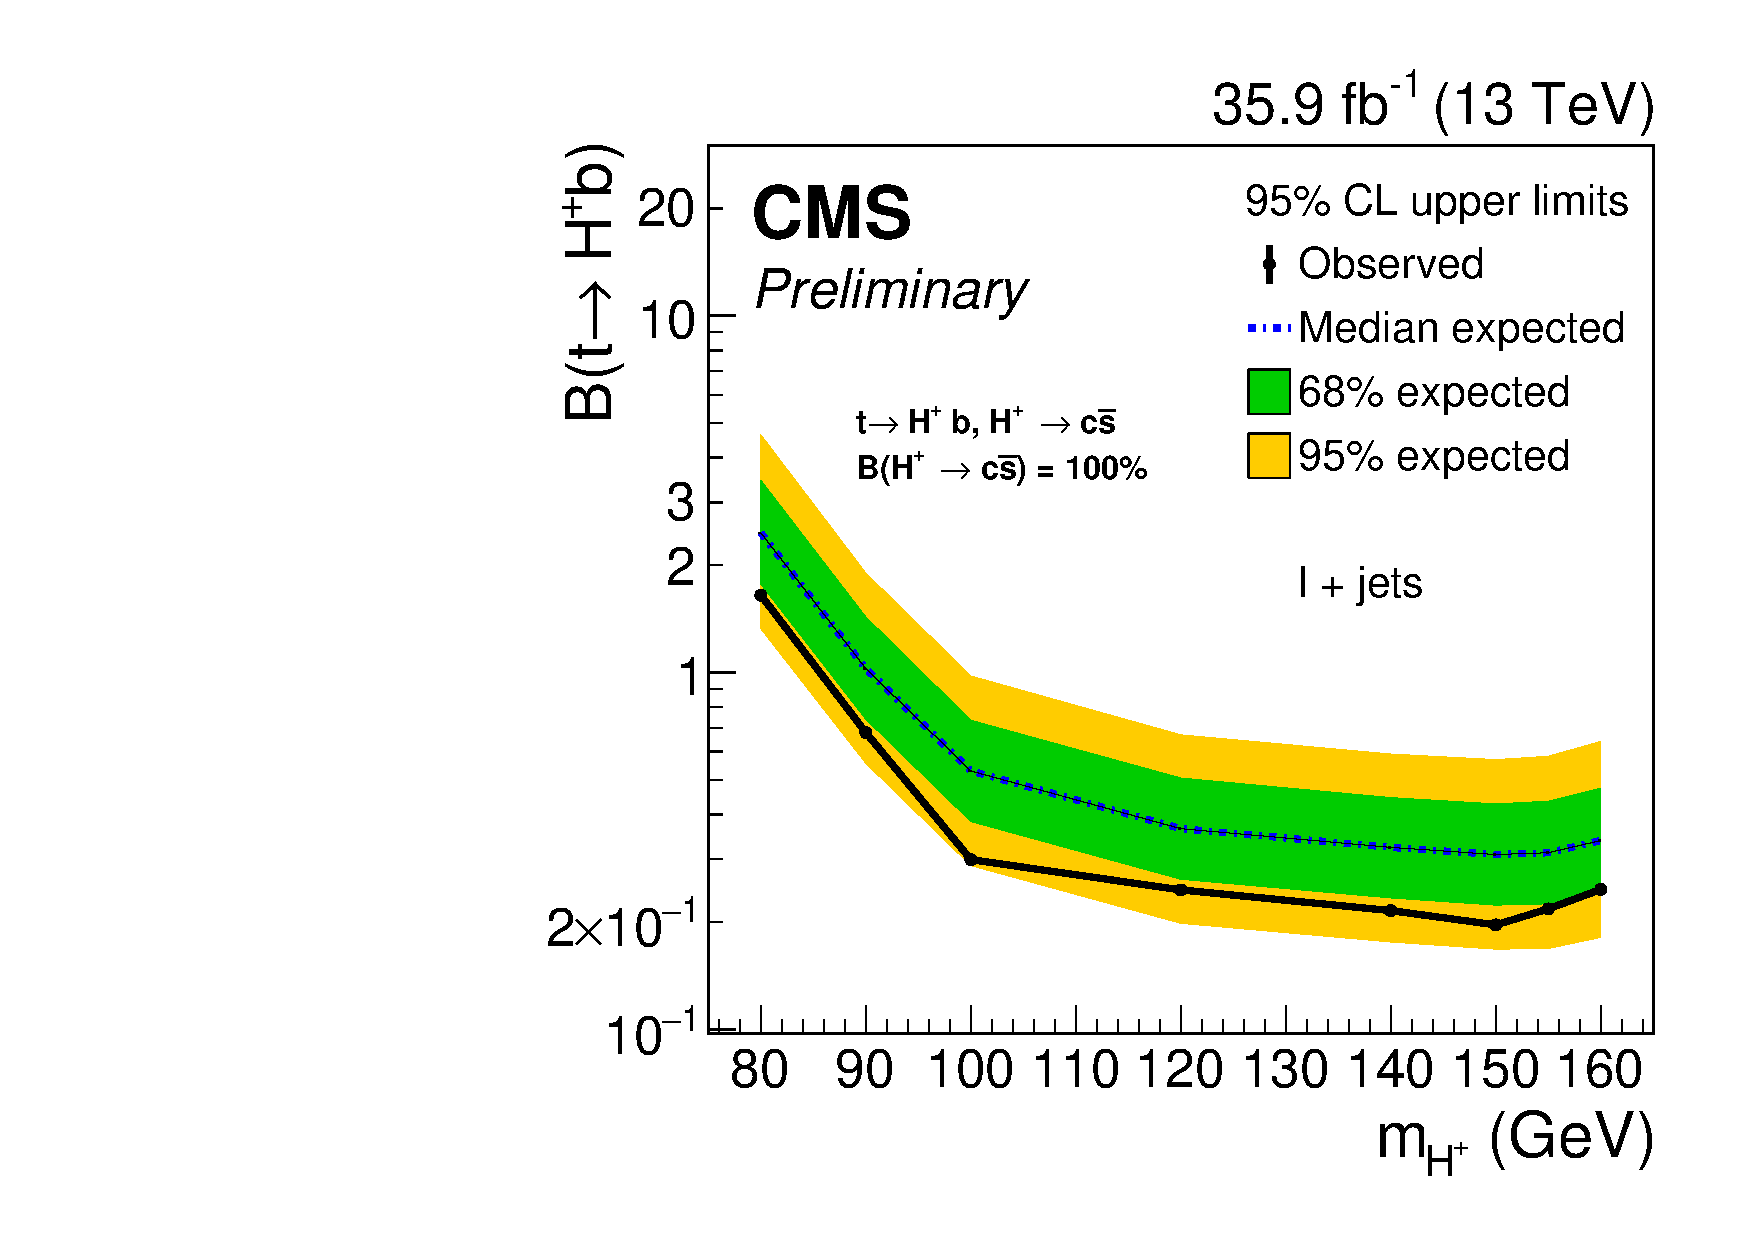
\includegraphics[width=0.55\textwidth]{Image/limit_mu_ele_Cat3_cTagEx.pdf}
    \caption{The expected and observed upper limits in \% on $\mathcal{B}(\PQt \to \PSHp\PQb)$ as a function
    of $m_{\PSHp}$ using \mjj after the individual charm tagging categories have been combined, for the muon +
    jets (upper left), electron + jets (upper right), and combined (bottom) channels.}
 \label{fig:limitPlot}
\end{figure}

\begin{table}[ht]
\centering
\topcaption{Expected and observed 95\% \CL exclusion limits in \% on $\mathcal{B}(\PQt \to \PSHp\PQb)$ for the muon (electron) channel, after the
individual charm tagging categories have been combined.}
\label{tab:limit_muon_ele}
\cmsTable{
\begin{tabular}{ccccccc}
\hline
\hline
\multirow{2}{*}{$m_{\PSHp}$ (\GeVns)} & \multicolumn{5}{c}{Expected} & \multirow{2}{*}{Observed} \\
& $-2\sigma$ & $-1\sigma$ & median & $+1\sigma$ & $+2\sigma$ &\\ \hline
\hline
80  & 1.62 (1.97) & 2.18 (2.63) & 3.06 (3.66) & 4.31 (5.14) & 5.85 (6.89) & 2.12 (3.29) \\
90  & 0.72 (0.80) & 0.96 (1.07) & 1.34 (1.48) & 1.87 (2.07) & 2.49 (2.77) & 0.79 (1.45) \\
100 & 0.36 (0.43) & 0.49 (0.56) & 0.68 (0.78) & 0.94 (1.09) & 1.25 (1.45) & 0.38 (0.61) \\
120 & 0.25 (0.29) & 0.33 (0.38) & 0.46 (0.53) & 0.64 (0.73) & 0.86 (0.97) & 0.29 (0.53) \\
140 & 0.22 (0.24) & 0.30 (0.32) & 0.41 (0.45) & 0.57 (0.62) & 0.75 (0.83) & 0.33 (0.35) \\
150 & 0.21 (0.24) & 0.28 (0.31) & 0.39 (0.44) & 0.54 (0.61) & 0.72 (0.81) & 0.37 (0.27) \\
155 & 0.22 (0.23) & 0.30 (0.31) & 0.41 (0.43) & 0.58 (0.61) & 0.77 (0.81) & 0.45 (0.27) \\
160 & 0.23 (0.26) & 0.31 (0.35) & 0.44 (0.49) & 0.62 (0.69) & 0.84 (0.94) & 0.44 (0.33) \\
\hline
\end{tabular}
}
\end{table}

\begin{table}[ht]
\centering
\topcaption{Expected and observed 95\% \CL exclusion limits in \% on $\mathcal{B}(\PQt \to \PSHp\PQb)$, after the
individual charm tagging categories and the electron and muon channels have been combined.}
\label{tab:limit_lepton}
\begin{tabular}{ccccccc}
\hline
\hline
\multirow{2}{*}{$m_{\PSHp}$ (\GeVns)} & \multicolumn{5}{c}{Expected} & \multirow{2}{*}{Observed} \\
& $-2\sigma$ & $-1\sigma$ & median & $+1\sigma$ & $+2\sigma$ & \\ \hline
\hline
80  & 1.33 & 1.77 & 2.46 & 3.45 & 4.63 & 1.65\\
90  & 0.56 & 0.74 & 1.03 & 1.43 & 1.90 & 0.68\\
100 & 0.29 & 0.38 & 0.53 & 0.73 & 0.98 & 0.30\\
120 & 0.20 & 0.26 & 0.36 & 0.51 & 0.67 & 0.25\\
140 & 0.18 & 0.23 & 0.32 & 0.45 & 0.59 & 0.21\\
150 & 0.17 & 0.22 & 0.31 & 0.43 & 0.57 & 0.20\\
155 & 0.17 & 0.22 & 0.31 & 0.44 & 0.58 & 0.22\\
160 & 0.18 & 0.24 & 0.34 & 0.47 & 0.64 & 0.25\\
\hline
\end{tabular}
\end{table}


%%%%%%%% SUMMARY %%%%%%%%%%%%%%%%%%%%%
\section{Summary}
\label{s:secConcl}
A search for a light charged Higgs boson \PHpm has been performed in the muon + jets
and electron + jets channels at $\sqrt{s}$ = 13\TeV, using a data sample with an integrated luminosity of
35.9\fbinv. The observed and predicted number of events are in agreement
within the statistical and systematic uncertainties as shown in
Table~\ref{tab:eventYield}. In the absence of observed signal, an exclusion limit
at 95\% confidence level on the branching ratio $\mathcal{B}(\PQt \to \PSHp\PQb)$ has
been computed by assuming
$\mathcal{B}(\PSHp \to \PQc\PAQs) = 100\%$. The observed exclusion limits are
in the range, depending on the \PSHp mass, 0.29--2.12\%, 0.27--3.29\%, and 0.20--1.65\% for the muon + jets,
electron + jets, and combined channels, respectively. The expected exclusion limits from 13\TeV are better by a factor
of ${\approx}4$, as compared to those obtained from earlier CMS results at 8\TeV~\cite{Khachatryan:2015uua}.

\bibliography{auto_generated}
